\documentclass[12pt, %
openright, 
oneside,
a4paper,
brazil]{facom-ufu-abntex2}
\usepackage{xcolor}
% Definindo novas cores
\definecolor{verde}{rgb}{0.25,0.5,0.35}
\definecolor{jpurple}{rgb}{0.5,0,0.35}
% Configurando layout para mostrar codigos Java
\usepackage{listings}
\usepackage{acronym}
\usepackage{longtable}
\lstset{
  language=Java,
  basicstyle=\ttfamily\small, 
  keywordstyle=\color{jpurple}\bfseries,
  stringstyle=\color{red},
  commentstyle=\color{verde},
  morecomment=[s][\color{blue}]{/**}{*/},
  extendedchars=true, 
  showspaces=false, 
  showstringspaces=false, 
  numbers=left,
  numberstyle=\tiny,
  breaklines=true, 
  backgroundcolor=\color{cyan!10}, 
  breakautoindent=true, 
  captionpos=b,
  xleftmargin=0pt,
  tabsize=4
}
\autor{Patrick Godinho} %TCC
\data{2015}
\orientador{Dr. Lásaro J. Camargos} %TCC
%\coorientador{Algum?} %TCC 


\usepackage{todonotes}


% ---
% Informações de dados para CAPA e FOLHA DE ROSTO
% ---

\titulo{PheroCast App} %TCC

\hypersetup{pdfkeywords={palavra 1}{palavra 2}{palavra 4}{palavra 4}{palavra 5}} %TCC

\begin{document}

\frenchspacing 

% ----------------------------------------------------------
% ELEMENTOS PRÉ-TEXTUAIS
% ----------------------------------------------------------
%\pretextual
\imprimircapa
\imprimirfolhaderosto


% ---
% Inserir folha de aprovação
% ---
%
% \includepdf{folhadeaprovacao_final.png} %TCC: depois de aprovado o trabalho, descomente esta linha e comente o próximo bloco para incluir scan da folha de aprovação.
%
\begin{folhadeaprovacao}

  \begin{center}
    {\ABNTEXchapterfont\large\imprimirautor}

    \vspace*{\fill}\vspace*{\fill}
    {\ABNTEXchapterfont\bfseries\Large\imprimirtitulo}
    \vspace*{\fill}
    
    \hspace{.45\textwidth}
    \begin{minipage}{.5\textwidth}
        \imprimirpreambulo
    \end{minipage}%
    \vspace*{\fill}
   \end{center}
    
   Trabalho aprovado. \imprimirlocal, 5 de janeiro de 2015: %TCC:

   \assinatura{\textbf{\imprimirorientador} \\ Orientador}  
   \assinatura{\textbf{Dr. Luis Fernando Faina}}% \\ Convidado 1} %TCC:
   \assinatura{\textbf{Me. Cláudio Camargo Rodrigues}}% \\ Convidado 2} %TCC:
   %\assinatura{\textbf{Professor} \\ Convidado 3}
   %\assinatura{\textbf{Professor} \\ Convidado 4}
      
   \begin{center}
    \vspace*{0.5cm}
    {\large\imprimirlocal}
    \par
    {\large\imprimirdata}
    \vspace*{1cm}
  \end{center}
  
\end{folhadeaprovacao}
% ---


%%As seções dedicatória, agradecimento e epígrafe não são obrigatórias.
%%Só as mantenha se achar pertinente.

% ---
% Dedicatória
% ---
\begin{dedicatoria}
   \vspace*{\fill}
   \centering
   \noindent
   \textit{Dedico a meu pai Paulo Sergio de Jesus Oliveira que sempre foi um exemplo de perseverança na minha vida!}  %TCC:
   \vspace*{\fill}
\end{dedicatoria}
% ---

% ---
% Agradecimentos
% ---
\begin{agradecimentos}
Agradeço a Deus, minha esposa e ao meu orientador Lásaro J. Camargos pelo apoio e dedicação para que eu conseguisse chegar ao final deste trabalho. %TCC:
\end{agradecimentos}
% ---

% ---
% Epígrafe
% ---
%\begin{epigrafe}
%    \vspace*{\fill}
%	\begin{flushright}
%		\textit{``Alguma citação que ache conveniente? \lipsum[10]''} %TCC:
%	\end{flushright}
%\end{epigrafe}
% ---



\begin{resumo} %TCC:

Nós  em redes móveis se movimentam e interagem eentre si e com a infraestrutura, ações que complicam a gestão da rede. Se a infraestrutura puder estimar a posição futura dos nós, com alto grau de acerto, tal estimativa poderia ser usada para, de forma proativa, reagir à movimentação dos nós, bem como tornar possível diversos serviços, como previsão de congestionamento, otimização de recursos de rede, e planejamento de rotas colaborativo. Há na literatura algoritmos para tal fim, prever a posição de nós em redes móveis, contudo, os mesmos carecem de validação utilizando dados reais. Neste trabalho propusemos e implementamos um aplicativo para telefones móveis que coleta rastros de mobilidade entre redes sem fio, que pode ser usado para avaliação de algoritmos de predição de mobilidade. O aplicativo desenvolvido foi testado por cinco usuários, por um período de um mês, levando à coleta de cerca de 50.000 registros de localização, e embora os rastros obtidos possam ser limitados de diversas formas, são já suficientes para exemplificar análises que podem ser feitas sobre tais conjuntos de dados.

 \vspace{\onelineskip}
    
 \noindent
 \textbf{Palavras-chave}: MANET, VANET, Android, Predição de Localização%TCC:
\end{resumo}

% ---
% inserir lista de ilustrações
% ---
\pdfbookmark[0]{\listfigurename}{lof}
\listoffigures*
\cleardoublepage
% ---

% ---
% inserir lista de tabelas
% ---
\pdfbookmark[0]{\listtablename}{lot}
\listoftables*
\cleardoublepage
% ---

% ---
% inserir lista de abreviaturas e siglas
% ---
%\begin{siglas} %TCC:
%  \item[Fig.] Area of the $i^{th}$ component
%  \item[456] Isto é um número
%  \item[123] Isto é outro número
%  \item[Zézão] este é o meu nome
%\end{siglas}
% ---

%% ---
%% inserir lista de símbolos, se for adequado ao trabalho. %TCC:
%% ---
%\begin{simbolos}
%  \item[$ \Gamma $] Letra grega Gama
%  \item[$ \Lambda $] Lambda
%  \item[$ \zeta $] Letra grega minúscula zeta
%  \item[$ \in $] Pertence
%\end{simbolos}
%% ---

% ---
% inserir o sumario
% ---
\pdfbookmark[0]{\contentsname}{toc}
\tableofcontents*
\cleardoublepage
% ---


\chapter*{Lista de abreviaturas}
\begin{acronym}
\acro{WiFi}{Wireless Fidelity}
\acro{SSID}{Service set ID}
\acro{BSSID}{Basic Service set Identifier}
\acro{API}{Application Programming Interface}
\acro{MANET}{Mobile Ad-Hoc Networks}
\acro{VANET}{Vehicular Ad Hoc Networks}
\acro{dBm}{decibel miliwatt}
\acro{LAN}{Local Area Network}
\acro{WAN}{Wired Area Network}

\end{acronym}


% ----------------------------------------------------------
% ELEMENTOS TEXTUAIS
% ----------------------------------------------------------
\textual


% ----------------------------------------------------------
% Introdução
% ----------------------------------------------------------

\chapter{Introdução}
\addcontentsline{toc}{chapter}{Introdução}
%TCC:
\section{Contextualização}
\subsection{Mobile Ad-hoc Network}
Uma \ac{MANET} é uma rede em que nós se movimentam livremente comunicando entre si e com o ambiente em que estão inseridos, sem a necessidade de nenhuma infraestrutura de rede. Essas interações abrem um leque de funcionalidades a serem implementadas para operar nesse meio. Como por exemplo, a funcionalidade que temos hoje em dia de rotear a internet do celular provinda de pacote de dados, com dispositivos próximos através de uma rede \ac{WiFi}.

Os nós em uma \ac{MANET} se movem arbitrariamente, e essa é a principal característica da rede, a qual torna a comunicação disponibilizada nesse ambiente complexa de se manter a qualidade das trocas de mensagens, pois o meio em que estão inseridos deve sempre estar se adaptando para as novas localizações em que os nós se encontram. \cite{de2002mobile}.

Desde que surgiu, a \ac{MANET} tem sido vista como uma das mais desafiantes abordagens de redes móveis tanto pela promessa do crescimento de dispositivos móveis, quanto pela sua complexidade, o que impulsionou a pesquisa envolvendo esse paradigma. A partir das pesquisas intensas nas \ac{MANET}, surgiram outras redes móveis baseadas em sua proposta inicial. Como por exemplo a \ac{VANET} que será introduzida na próxima seção.



\subsection{VANET}
\ac{VANET} são redes móveis \ac{MANET} onde os nós são os veículos e até a estrada, onde há comunicação apenas entre os automóveis (IVC - Inter Vehicle Communication), ou entre os mesmos e a estrada (RVC - Road Vehicle Communication). \cite{ufrj-Vanet}

Assim como na MANET, a Vehicular Ad-Hoc Network também permite que várias aplicações com vários objetivos sejam desenvolvidos, como por exemplo alertar obstáculos na estrada, broadcast de informações de segurança, compartilhar informações de tráfego ou até solicitar socorro em algum acidente.

As simulações e experimentos dos algoritmos tem tido um papel importante no desenvolvimento das soluções para redes veiculares. A atenção maior tem sido dada no desenvolvimento de modelos realistas da estrada e principalmente no estudo da mobilidade dos veículos. Por exemplo, modelos de como os carros se movem ao longo do trajeto, levando em consideração sua velocidade, sinais de trânsito, dentre outros fatores. \cite{6710069} 

O grande desafio das Redes Ad-Hoc Veiculares é o roteamento entre os nós, devido à alta taxa de mobilidade dos veículos que são conectados entre si intermitentemente, dificultando a entrega das mensagens entre os nós e a comunicação com a estrada, pois frequentemente um nó muda seu endereço ficando assim diferente de qual se identificou.

Além do problema citado acima, existe um agravante relacionado a velocidade de conexão entre os nós, os quais se comunicam muito rápido, levando em consideração que os mesmos estejam em uma via rápida.

\subsection{Predição de localização}
Estudar a implementação de algoritmos que preveem a localização de um nó em um determinado momento é de extrema importância, pois impulsiona e otimiza a utilização das redes \ac{MANET}, bem como as pesquisas relacionadas à estas redes e suas derivadas através da gestão proativa que será exemplificada a seguir.  \cite{6838650}

Caso um nó mande uma requisição para outro e logo após mude de localização, os algoritmos possibilitam o responsável pela resposta ser proativo o bastante para saber em qual posição o destinatário estará para receber a mensagem. Com a implementação da predição, grande parte do problema da mobilidade o qual é o principal desafio da \ac{VANET} estaria resolvido.

Podemos descrever vários cenários de utilização da predição de localização, operações como prever e otimizar tráfego em cidades inteligentes, estudo de potenciais clientes para um passeio ecológico, alertas de acidentes na estrada em veículos inteligentes.

\subsubsection{PheroCast}
PheroCast é o nome que se deu uma abordagem de previsão da localização futura de um nó em uma rede ad-hoc móvel. Foi nomeado assim pela semelhança com o fenômeno que acontece na colônia das formigas, o qual para alertar problemas ou marcar o caminho, por onde a formiga passar ela deixará um rastro, formando assim um caminho.

Nessa abordagem, o algoritmo de previsão é desenvolvido para ser processado nos próprios nós móveis. Assim, a cada intervalo de tempo definido, o nó registra um rastro de onde está. Daí vem a semelhança com o ``Pheronomium'' deixado no rastro por onde a formiga passa.

Assim, com o grafo representando o histórico dos ``traces'' de um determinado nó, é possível determinar uma probabilidade de onde ele estará em determinado momento a partir de um certo lugar.


Segundo \cite{fynn} foi feita uma avaliação do algoritmo PheroCast usando os caminhos dos ônibus de Seattle Metro Transit, e através dos resultados apresentados para 186 viagens ao longo da rota 007, a qual registrou 310206 ``traces'', as suposições de que os nós seguem padrões claros foi validada. Foi descoberto que a abordagem obteve bons resultados em relação à predição das futuras posições dos ônibus. A avaliação obteve 96,25\% de resultados positivos. 


O grande problema do PheroCast é a sua avaliação limitada, ou seja, é necessário, para uma abordagem com essas características, uma avaliação extensa com dados reais, que simulam de verdade a mobilidade humana. 

Atualmente não existem ``traces'' reais, e sim módulos de mobilidade sintéticos, os quais não são realistas. Daí vem a proposta deste trabalho, o qual irá cooperar para avaliação confiável do PheroCast, coletando dados de mobilidade humana reais, através de seus dispositivos móveis.

\section{Proposta}
A proposta deste trabalho é desenvolver um aplicativo que opere em dispositivos móveis com sistema operacional Android, para capturar \emph{traces} reais de mobilidade humana. Para tal, o sistema irá coletar, periodicamente, diversas informações disponíveis sobre as redes wireless que estão no alcance do dispositivo móvel do usuário, e armazenar em um servidor para que os dados sejam compilados e utilizados para avaliação do PheroCast.

Para que a coleta resulte em rastros úteis, a mesma deve ser feita com um grande número de usuários, coletando assim uma variação importante de informações que serão utilizadas nos diversos tipos de análise. 


\chapter{Referencial Teórico}
\section{PheroCast}

	O PheroCast, conjunto de algoritmos para prever a localização de um nó em alguma rede móvel, foi desenvolvido por um grupo de pesquisa da Universidade Federal de Uberlândia, o The Distributed Systems and Networks  Research Group, criado em 2013, constituído de doutores, mestres e alunos da Faculdade de Computação. citar grupo. 
	
	
	Para entendermos a abordagem do Pherocast, que consiste na previsão da posição dos nós de uma rede móvel baseada no conceitos dos feromônios, vamos conceituar e exemplificar alguns componentes utilizados pelo algoritmo.

	Como as formigas passam a vida em contato com o solo, em suas caminhadas, elas deixam um rastro de feromônio que pode ser seguida por ouras formigas. Trazendo para o nosso contexto, um nó em uma rede móvel pode sinalizar os pontos em que passou, e assim construir um caminho que percorreu de um ponto a outro. Podemos também afirmar com esse conceito que um nó está em uma localização X se X é o sinal mais perto de sua posição.
	
	Cada marca, ou log deixado pelo nó contém a informação da localização e a hora em que passou por ele, e a direção tornando assim análises como a velocidade do nó, ou a grandeza da localização. Por exemplo, caso um nó sinalize que está em uma localização em vários intervalos de tempo consecutivos, podemos concluir que essa localização, ou área de alcance é grande, ou que o nó está em baixa velocidade. Por outro lado, caso uma localização seja pouco marcada, o nó pode estar em uma alta velocidade ou a área é pequena, onde pouco ``feromônio'' foi liberado.\cite{6838650} 
	
	No PheroCast esses sinais que contém a localização e a hora são convertidos em Phero Trails, um dígrafo que contém como vértices os locais visitados pelos nós, e a direção em que estão (norte, sul, leste, oeste) ligados  por arestas de forma em que represente a movimentação do nó, e assim seu caminho o qual possui uma localização inicial e uma final.\cite{6838650} 
	
	Com os Phero Trails definidos, temos a capacidade de utilizar um dos algoritmos do PheroCast e traçar o que chamamos de Phero Maps, dígrafos que contém além da localização e a direção, a quantidade de vezes que o nó passou por ali, ligados por arestas que indicam a próxima localização que o nó passou, e assim por diante. Assim conseguimos concluir que para chegar em uma localização final, o nó passou por diversos caminhos diferentes, também definimos as possíveis rotas entre um determinado ponto e outro.\cite{6838650} 
	
	Dado um Phero Map definido, temos todas as variáveis que o algoritmo de previsão de uma futura localização do nó, descrita no Phero Cast necessita. Tais elas são: localização, direção, quantidade de vezes que passou pela localização. 
	
 	O produto final desse trabalho, tem como objetivo produzir dados reais de localização, tratando os feromônios como registros de rede \ac{WiFi}, registrados pelo dispositivo móvel em um determinado intervalo de tempo, e armazenando em um local para ser reproduzidas em mapas e diagramas, como aborda o Phero Cast.

\section{Redes sem fio}
A troca de mensagens digitais utilizando redes sem fios é uma ideia bem antiga, pois em 1901, foi demonstrado como funcionava um telégrafo sem fio, por Guglielmo Marconi, que transmitia informações de um navio para o litoral por meio de código morse. A grande diferença para a tecnologia atual é o desempenho, mas a teoria da funcionalidade apresentada com os aparelhos que temos hoje em dia é a mesma. Nesse paradigma, o mestre gerencia toda a comunicação com os escravos, parâmetros como endereço, tempo 

Seguindo o modelo de \cite{tanenbaum2003redes} iremos dividir as redes sem fio em três principais categorias. A primeira categoria é a interconexão de sistemas define-se por usar rádio para interconectar periféricos de um computador como monitor, teclado, mouse, impressora. Hoje em dia alguns usuários têm dificuldade para conectar os cabos à unidade principal, outros preferem por estética e organização não utilizar cabos em suas estações. Para resolver esses e outros detalhes, algumas empresas se juntaram para desenvolver uma rede sem fio de alcance limitado nomeada Bluetooth.

Essa categoria de rede utiliza uma arquitetura de mestre-escravo conforme ilustrado na Figura 1, como por exemplo no cenário do computador e seus periféricos, na maioria das vezes o CPU é o mestre, e os componentes como mouse, teclado, impressora, fone, os escravos. Nesse paradigma, o mestre é responsável por gerenciar a comunicação com os periféricos, dizendo qual endereço utilizar, o período de transmissão, a frequência a ser utilizada, dentre outros parâmetros.

\begin{figure}[hbt]
  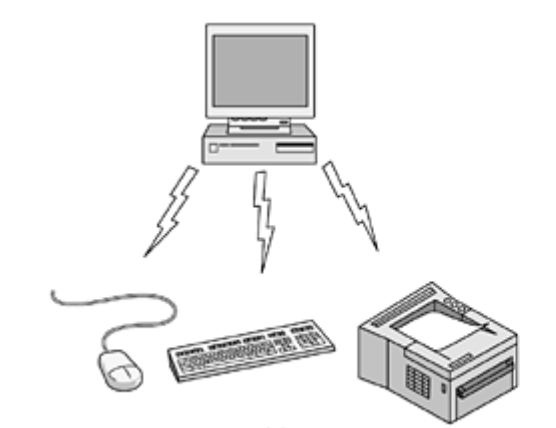
\includegraphics[scale=0.9]{bt}
  \caption{Paradigma Mestre-Escravo \cite{tanenbaum2003redes}}
\end{figure}

A segunda categoria de redes sem fio são as LANs sem fios. Definidas por arquiteturas em que todo computador, ou dispositivo inserido na rede tem um modem de rádio e uma antena que fornece um meio de comunicar com outros dispositivos. Na maioria das vezes existe uma antena principal que fornece a comunicação para os computadores conectados na mesma. Como por exemplo na Figura 2, que demonstra a arquitetura comum das \ac{LAN} sem fios que temos hoje na maioria das casas.

\begin{figure}[hbt]
  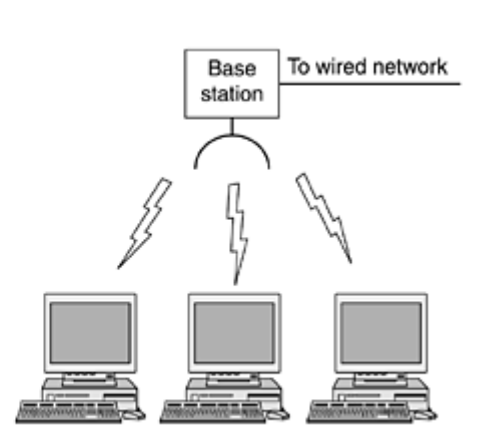
\includegraphics[scale=0.9]{lan} 
  \caption{Arquitetura comum de uma \ac{LAN} sem fio \cite{tanenbaum2003redes}}
\end{figure}

As \ac{WAN} sem fio, terceira categoria de redes sem fio, é utilizada em sistemas geograficamente distribuídos como por exemplo a rede de telefonia celular. Existe uma grande semelhança entre as redes sem fio \ac{LAN} e \ac{WAN}, uma das diferenças mais evidentes são as distâncias de alcance do sinal, implicando na taxa de velocidade de comunicação. Ou seja, como nas \ac{WAN} sem fio a distância é maior, a velocidade de tráfego dos bits é bem menor que nas \ac{LAN} que a velocidade pode alcançar entre 10Mbps e 1Gbps.

Para fornecer acesso a arquivos, à Internet, a maioria das redes sem fio se conecta   em algum ponto com a rede com fio. Para isso, existem vários tipos de conexões, que são desenhadas conforme a necessidade. Como por exemplo na Figura 3, onde um avião com acesso a internet é ilustrado. Na aeronave existe um único roteador ligado com algum roteador em terra firme, e conforme o percurso os equipamentos  que não estão voando são trocados.

\begin{figure}[hbt]
  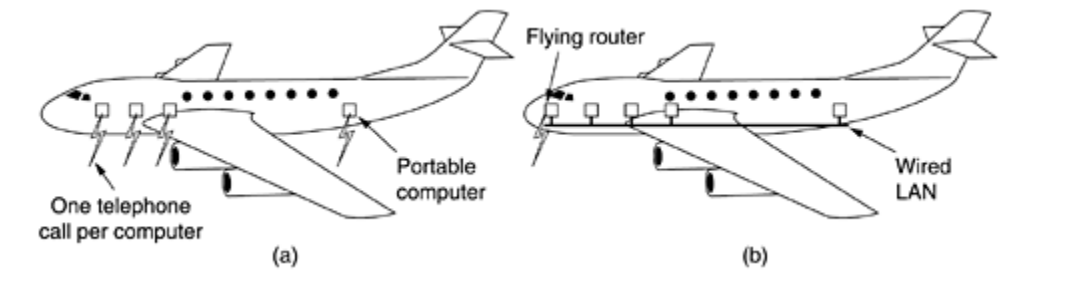
\includegraphics[scale=0.9]{aviao}
  \caption{Exemplo de avião com internet \cite{tanenbaum2003redes}}
\end{figure}



\section{Android}

	Para o desenvolvimento desse trabalho, utilizamos o sistema operacional Android, baseado em Linux que opera em celulares, netbooks, tablets, dentre outros dispositivos. O Android nos fornece um robusto framework de aplicação que nos permite implementar aplicações para dispositivos móveis utilizando Java.
	
	Tal framework disponibiliza alguns componentes, os quais alguns deles foram utilizados na construção desse trabalho.
	Iremos detalhar cada componente a seguir:
	\cite{googleand}
	
	\subsection{Activities}
	A Activity é o componente responsável por fazer o bootstrap do aplicativo, ou seja, tem o papel de gerenciar as primeiras ações do app. Para isso utiliza-se do seu ciclo de vida, tal conceito ilustrado na Figura 4.
	
	O componente Activity representa uma única tela com interface para o usuário. Por exemplo, imaginemos um aplicativo de lista de compras, iremos ter uma Activity para exibir a lista de compras, outra activity para adicionar um novo produto na lista de compras, e outra para exibir um relatório de quanto gastamos no mês.
	Uma Activity é implementada no código do aplicativo extendendo a classe Activity do Android.
	
	\begin{figure}[hbt]
  		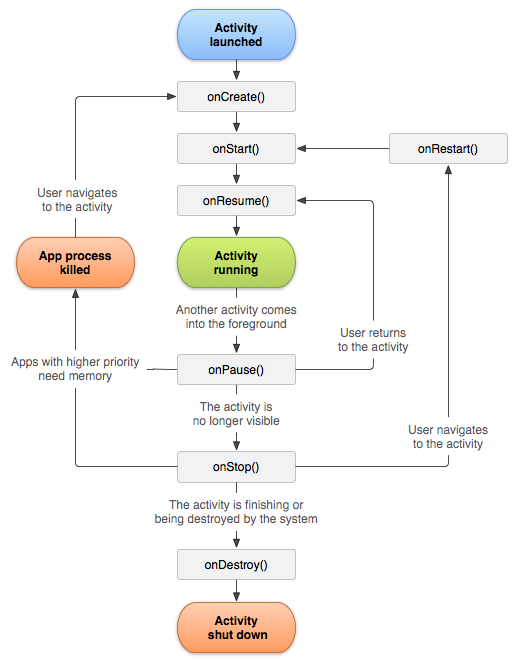
\includegraphics [scale=.7] {activity_lifecycle}
  		\caption{Ciclo de vida de uma Activity \cite{docAndroid}}
	\end{figure}

	
	\subsection{Services}
	Service é o componente que roda em background no Android, podendo processar longas operações ou processar algum processo remoto. Um Service não é responsável por fornecer interface para o usuário. Para entendermos melhor o funcionamento do Service, podemos exemplificar com o processo de tocar música enquanto se navega em outro aplicativo.
	Um Service é implementado no código do aplicativo extendendo a classe Service do Android.\cite{docAndroid}
	
	\subsection{Content Providers}
	Os Content Providers são parte importantíssima da arquitetura de um sistema android. É responsabilidade deles prover às aplicações o conteúdo que elas precisam para funcionar, ou seja, os dados.

As aplicações poderiam muito bem acessar diretamente um banco de dados, por exemplo. Porém, é uma boa prática tornar o modo como os dados são gravados transparente à aplicação. 

Além disso, essa técnica permite a criação de Shared Content Providers, que são providers “públicos” que podem ser acessados por várias aplicações. Por exemplo, existe o content provider de SMS/MMS que permite a qualquer aplicação ler as mensagens recebidas por um telefone celular.

	\subsection{Broadcast receivers}
	O Broadcast Receiver é o componente responsável por receber as mensagens broadcast do Sistema Operacional, por exemplo anúncios de que a tela foi desligada, ou a bateria está com pouca carga, ou uma foto foi tirada, ou algo na rede foi alterado. Esse componente, não fornece telas para o usuário, mas é possível criar uma barra de notificação através dele.

	\subsection{Arquivo Manifest}
	Para que o Android consiga iniciar um componente da aplicação, o sistema deve saber que esse componente existe através do arquivo AndroidManifest.xml. A aplicação desenvolvida deve conter as declarações de todos os componentes nesse arquivo, o qual está sempre localizado na pasta raiz do projeto.		


\chapter{Proposta}


\section{Arquitetura}
A proposta principal desse trabalho é um aplicativo para plataformas Android que possibilita a coleta de informações de redes sem fio ao seu alcance, armazene-as e as envie à um banco de dados na internet. Para atender essa proposta, desenhamos uma arquitetura que consiste em duas partes, cliente e servidor.

 O cliente é responsável pela coleta dos dados e ocasionalmente enviará os dados ao servidor. O servidor deverá consumir os dados enviados pelo dispositivo  e armazenar em um banco de dados, como mostra na Figura 5.  A seguir detalhamos cada um das partes.

\begin{figure}[hbt]
  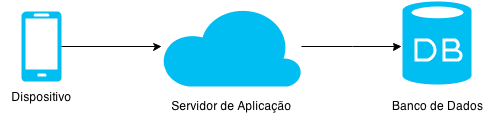
\includegraphics{arquiteturaProposta}
  \caption{Arquitetura Proposta}
\end{figure}


\subsection{Cliente}
Do lado do cliente desenvolvemos um sistema para rodar em dispositivos com o sistema operacional Android, utilizando a linguagem Java.

\begin{figure}[hbt]
  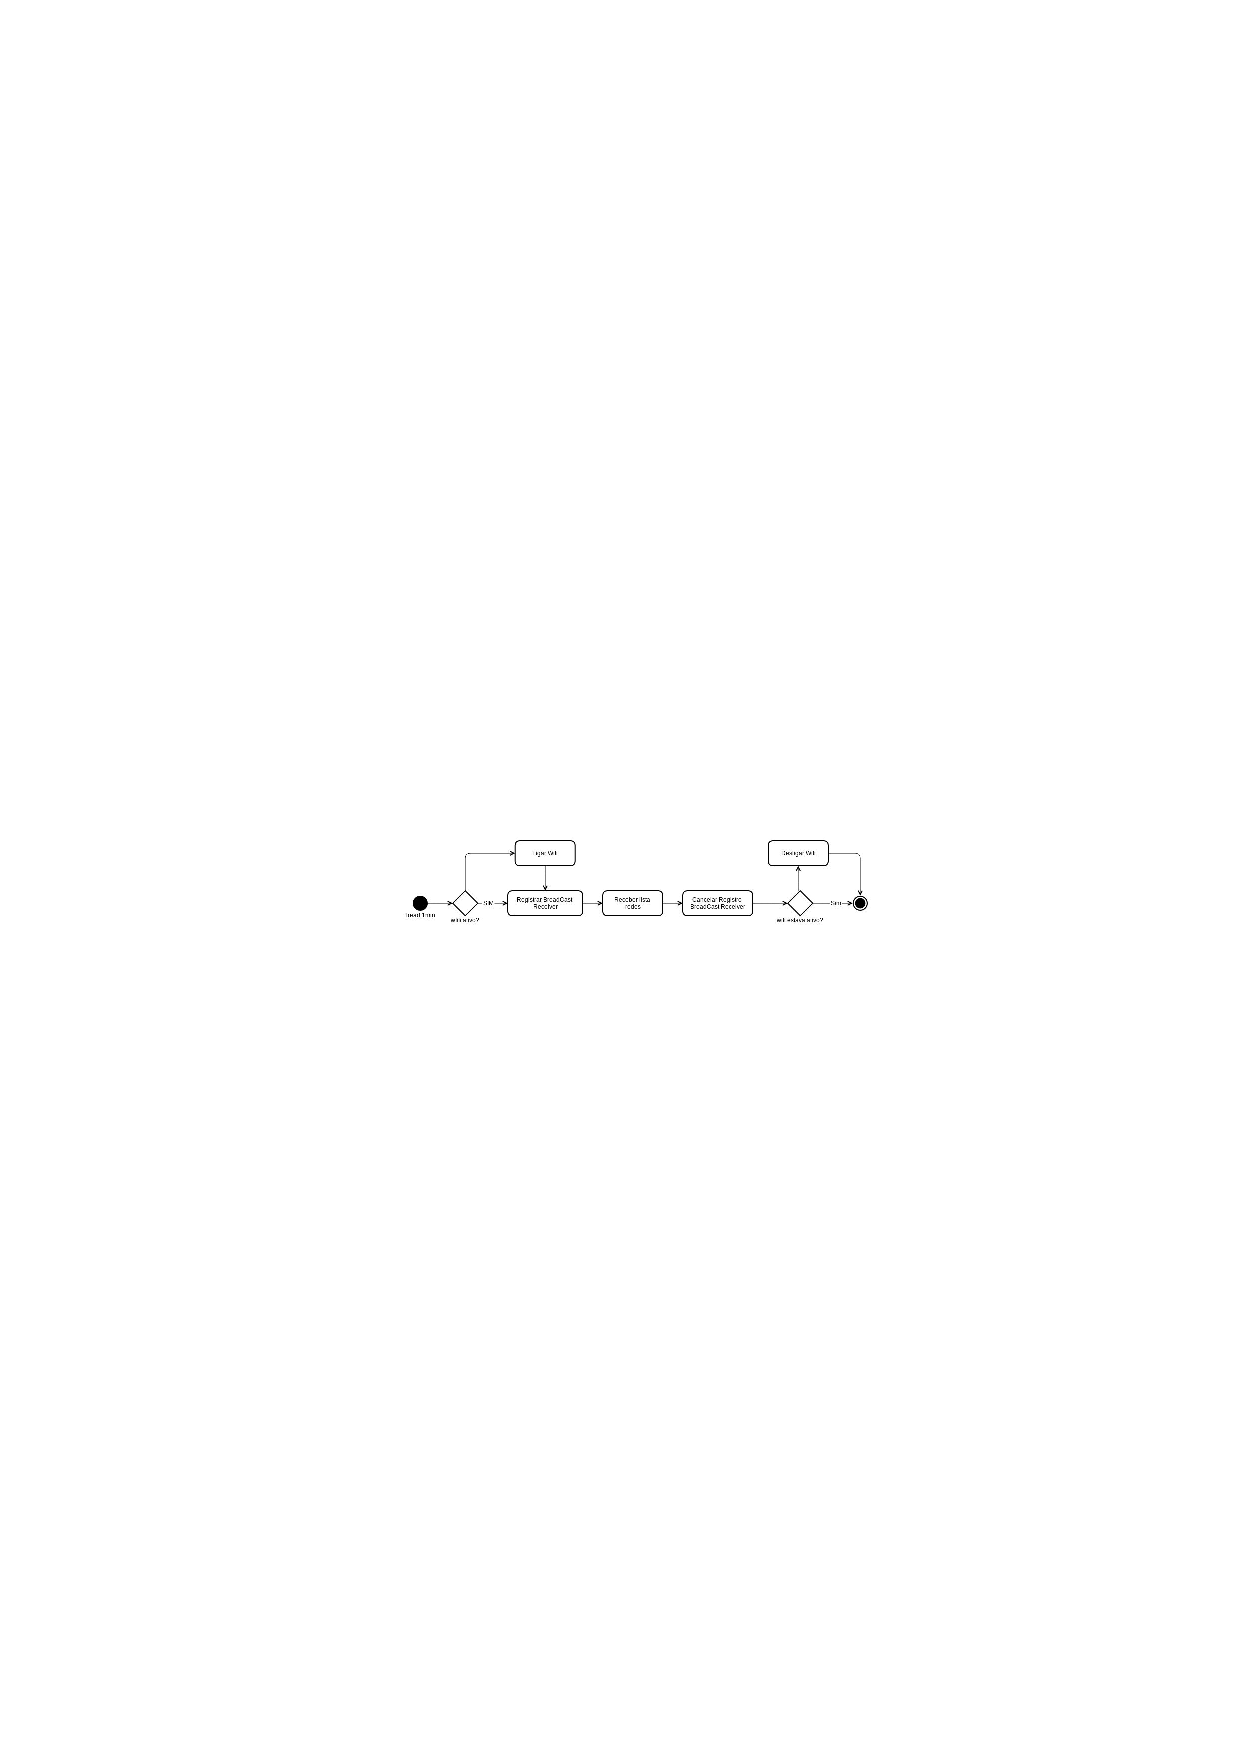
\includegraphics [scale=.4] {pherocast1}
  \caption{Processo de captura dos dados pelo aplicativo.}
\end{figure}

O aplicativo irá utilizar os serviços de \ac{WiFi} do aparelho para realizar a coleta dos pontos de rede que estão ao redor naquele determinado momento. Após a coleta, o sistema irá armazenar as informações coletadas na base de dados local do 	dispositivo, para isso utilizaremos o banco de dados SQLite. Tal procedimento é ilustrado na Figura 6.

Para realizar o envio ao servidor, o aplicativo será alertado quando o dispositivo se conectar a uma rede \ac{WiFi} com rede Internet, assim irá enviar os dados armazenados em sua base local para o servidor de aplicação na nuvem e apagar os mesmos. 

Caso o serviço de \ac{WiFi} esteja desligado, o aplicativo deverá ser responsável por após ligar o \ac{WiFi} e coletar os dados, desligar o mesmo, voltando assim para o estado inicial antes da coleta. Fazendo com que assim, não haja alteração no funcionamento do aparelho.




\subsection{Servidor}
Para o servidor, propomos utilizar algum servidor na nuvem de alta escalabilidade e alta disponibilidade, por se tratar de inserções contínuas todo o tempo.

O servidor deve tratar e  armazenar as informações que virão do cliente, como:
\begin{itemize}
  \item \ac{SSID} - Nome da rede.
  \item  \ac{BSSID} - MAC Address. 
  \item Capabilities - Características de segurança. 
  \item Frequency - Frequência do canal que o dispositivo utilizou na comunicação.
  \item Level - Intensidade do sinal em \ac{dBm}.
  \item Horário - Horário em que a rede foi capturada
  \item Identificador do Usuário do Dispositivo
  \end{itemize}
  
\subsection{Limpeza dos dados}
O sistema deverá tratar os dados do cliente com anonimidade, ou seja o aplicativo deve estar preparado para tratar a informação de identificação do usuário como um dado ilegível, ou melhor dizendo, não permitindo o usuário ser reconhecido. 

\chapter{Desenvolvimento}

\section{Aplicativo}
Como já mencionado, o produto final deste trabalho foi um aplicativo para dispositivos Android, o qual armazena periodicamente as informações das redes \ac{WiFi} disponíveis em seu alcance, e disponibiliza em um certo momento essas informações na nuvem.

Para tal, utilizamos a \ac{API} do Android para operações que envolveu o funcionamento do dispositivo, como por exemplo, a coleta das informações das redes em alcance, o sinal de que foi encontrado uma rede com internet, a ação de desligar e ligar o receptor \ac{WiFi} do aparelho, dentre outras operações. Além disso, implementamos o código orientado a objetos, onde cada rede coletada foi representada por um objeto.

Foram utilizadas também classes que auxiliam nas funcionalidades do aplicativo, como por exemplo, o armazenamento em uma base de dados do dispositivo, o envio dos dados para a nuvem, a identificação do usuário pelo e-mail cadastrado no dispositivo.

Abaixo detalharemos cada classe do código, com o objetivo de entendermos a estrutura do desenvolvimento do aplicativo.

Começaremos pela MainActivity, classe estendida do componente Activity do Android, o qual foi detalhado no nosso referencial teórico, que é a nossa principal classe, ou seja código responsável pela inicialização e processamento do aplicativo, através do método onCreate(). Esse método cria uma tarefa agendada que roda em intervalos de um minuto. Tal tarefa, é responsável por verificar a situação do \ac{WiFi} do aparelho, e, caso este esteja desligado, é ligado. Toda essa verificação do \ac{WiFi}, é feita no método getWifiState(). O trecho de código a seguir representa a implementação da tarefa.
\begin{lstlisting}
	protected void onCreate(Bundle paramBundle) {
		super.onCreate(paramBundle);
		setContentView(2130903064);
		wifi = ((WifiManager) getSystemService("wifi"));
		wifiReciever = new WifiScanReceiver();
		scanTask = new TimerTask() {
			public void run() {
				handler.post(new Runnable() {
					public void run() {
						getWifiState();
						registerReceiver(wifiReciever, new IntentFilter(
								"android.net.wifi.SCAN_RESULTS"));
						scanInitiated = true;
						wifi.startScan();
					}
				});
			}
		};
		t.schedule(scanTask, 300L, 60000L);
	}
\end{lstlisting}


  Após tratar a situação do sinal wireless do aparelho, a tarefa registra através de um Intent, a classe WifiScanReceiver estendida do componente BroadCastReceiver, responsável por receber o resultado da varredura das redes \ac{WiFi} ao alcance do aparelho realizada.
 
 A responsabilidade da coleta das redes sem fio é do objeto instanciado da classe WifiManager da \ac{API} do Android, o qual é executado através do método startScan(), após a tarefa registrar o receptor das redes encontradas.
 
  Ao receber a lista de redes através do método getScanResults da classe WifiManager, a classe WifiScanReceiver converte a lista recebida em um array de objetos da classe NetworkPoint, classe criada para representar a rede e seus atributos que são \ac{BSSID}, \ac{SSID}, Capabilities, Frequency, level e o momento em que foi capturada. O array de NetworkPoint é salvo na base de dados, utilizando a classe NetworkPointDAO, a qual, quando instanciada através do padrão de projeto Singleton, é criada em conjunto com a PersistenceHelper, para auxiliar nas operações com o banco de dados do aplicativo, o qual foi utilizado SQLite.
 
 Importante lembrar que após o serviço de receber e armazenar as redes capturadas, a situação anterior ao processamento do sinal wireless do aparelho é mantida, ou seja, caso o aparelho esteja com a funcionalidade \ac{WiFi} desligada, após o processamento (que liga a mesma), a tarefa principal é responsável por desligá-la. 
 
  Para armazenar na nuvem as informações das redes coletadas, foi utilizada a classe NetworkChangeReceiver, estendida do componente BroadCastReceiver, que tem como objetivo principal enviar um POST para o serviço de armazenamento caso o dispositivo conecte em alguma nova rede sem fio e que a mesma tenha acesso a internet. Para cada rede armazenada no dispositivo, uma requisição POST é realizada com a informação contendo o e-mail do usuário dono do dispositivo. Tal informação é adquirida através da classe UserEmailFetcher. Após o envio das informações da rede, a mesma é excluída da base de dados do aplicativo no dispositivo.

  O relacionamento entre as classes descritas acima pode ser melhor visualizado no diagrama de classes, representado na Figura 7.    
  
  \begin{figure}[hbt]
  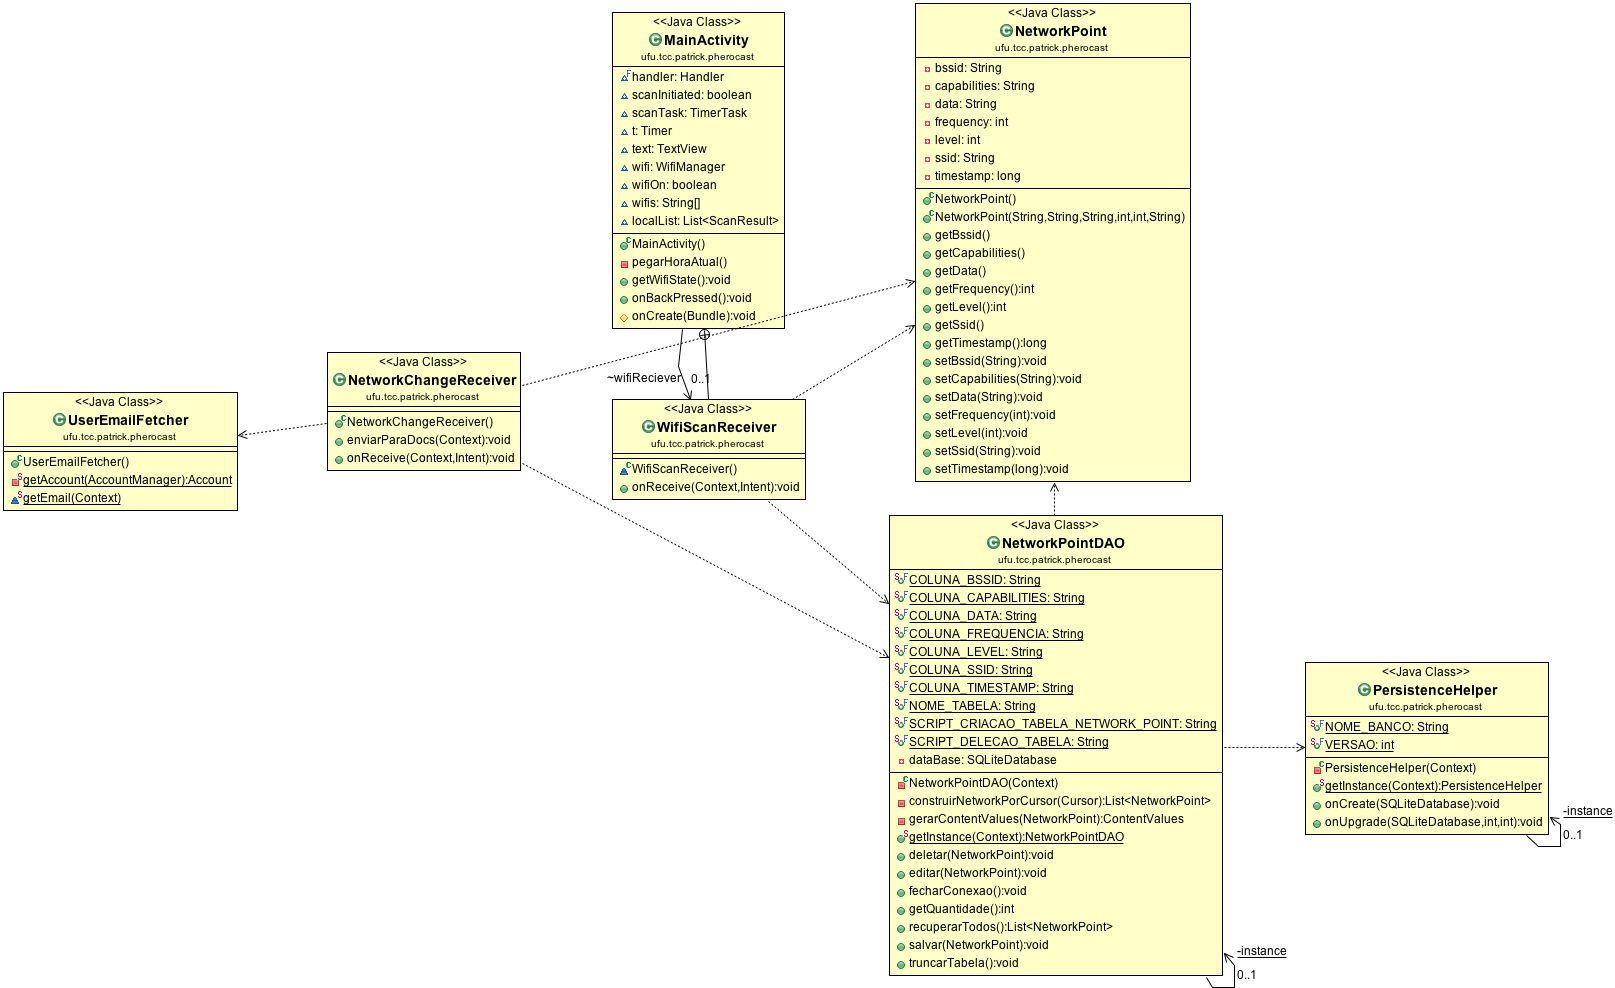
\includegraphics [scale=.3] {diagrama}
  \caption{Diagrama de classes do PheroCast APP}
\end{figure}
  

 \section{Google Docs}
Com o objetivo de implementar o serviço de armazenamento na nuvem, o serviço de armazenamento na nuvem, utilizamos o Google Docs, que é altamente disponível e gratuito, nos fornece um serviço de criação, edição e utilização de formulários, onde as respostas são armazenadas em planilhas compartilhadas. A Figura 8 exibe o formulário que foi criado para esse trabalho, onde cada campo representa um atributo da rede inserida.

Para armazenar as redes coletadas através desse formulário, foi necessário estudar o código e a requisição do botão ``submit'' do ``form'', em busca de algo que nos desse a possibilidade de automatizar as ações de digitar os dados de cada rede wireless coletada e clicar no botão enviar, para que assim o dado fosse inserido na planilha de resposta.

Ao estudar o tráfego de dados consequentes do clique no botão que representa o envio do formulário, identificamos a requisição POST realizada e coletamos as informações da mesma, dados como a URL requisitada e o formato dos dados enviados. 

O trecho de código a seguir, retirado da classe NetworkChangeReceiver, é disparado quando o aplicativo recebe a notificação que o aparelho conectou-se com a internet, e faz a iteração do array de redes sem fio que estão armazenadas no banco de dados do celular, e para cada rede é feita uma requisição POST ao Google Docs.


\begin{lstlisting}
	if (!localIterator.hasNext())
        return;
      NetworkPoint localNetworkPoint = (NetworkPoint)localIterator.next();
      String str1 = localNetworkPoint.getSsid();
      String str2 = localNetworkPoint.getBssid();
      String str3 = localNetworkPoint.getCapabilities();
      String str4 = String.valueOf(localNetworkPoint.getFrequency());
      String str5 = String.valueOf(localNetworkPoint.getLevel());
      String str6 = localNetworkPoint.getData();
      String str7 = UserEmailFetcher.getEmail(paramContext);
      localHttpRequest.sendPost("https://docs.google.com/forms/d/1G_dkyvwug--i_We7qAaA3QV-Xw_plTBJeKdElW22S4w/formResponse", "entry_2059700=" + URLEncoder.encode(str1) + "&" + "entry_1828317397=" + URLEncoder.encode(str2) + "&" + "entry_2146852893=" + URLEncoder.encode(str3) + "&" + "entry_312023197=" + URLEncoder.encode(str4) + "&" + "entry_644637792=" + URLEncoder.encode(str5) + "&" + "entry_604910793=" + URLEncoder.encode(str6) + "&" + "entry_612999935= " + URLEncoder.encode(str7));
      localNetworkPointDAO.deletar(localNetworkPoint);
\end{lstlisting}  

 Na linha 11 é feita a requisição POST, utilizando a URL do endereço destinatário, e os dados da chamada os quais representam os campos do formulário que será respondido a quantidade de vezes necessárias para esvaziar o banco de dados local. 
 
Resumindo e exemplificando, imaginemos um cenário onde o aplicativo coletou durante o dia seis mil redes ao seu redor e armazenou em sua base de dados local. Ao chegar a noite, o dispositivo conecta-se com uma rede \ac{WiFi} com Internet, então o aplicativo ao receber a notificação que está conectado a Internet, faz seis mil requisições ao Google Docs, respondendo ao formulário criado, onde cada resposta contém dados de uma única rede sem fio coletada.

Consideramos para trabalhos futuros a melhoria das requisições ao serviço de armazenamento, pois milhares de requisições seguidas não é o melhor procedimento a se realizar, e sim uma requisição com um lote de redes sem fio, diminuindo assim a quantidade de transações com o sistema de armazenamento na nuvem.
 
 
\begin{figure}[hbt]
  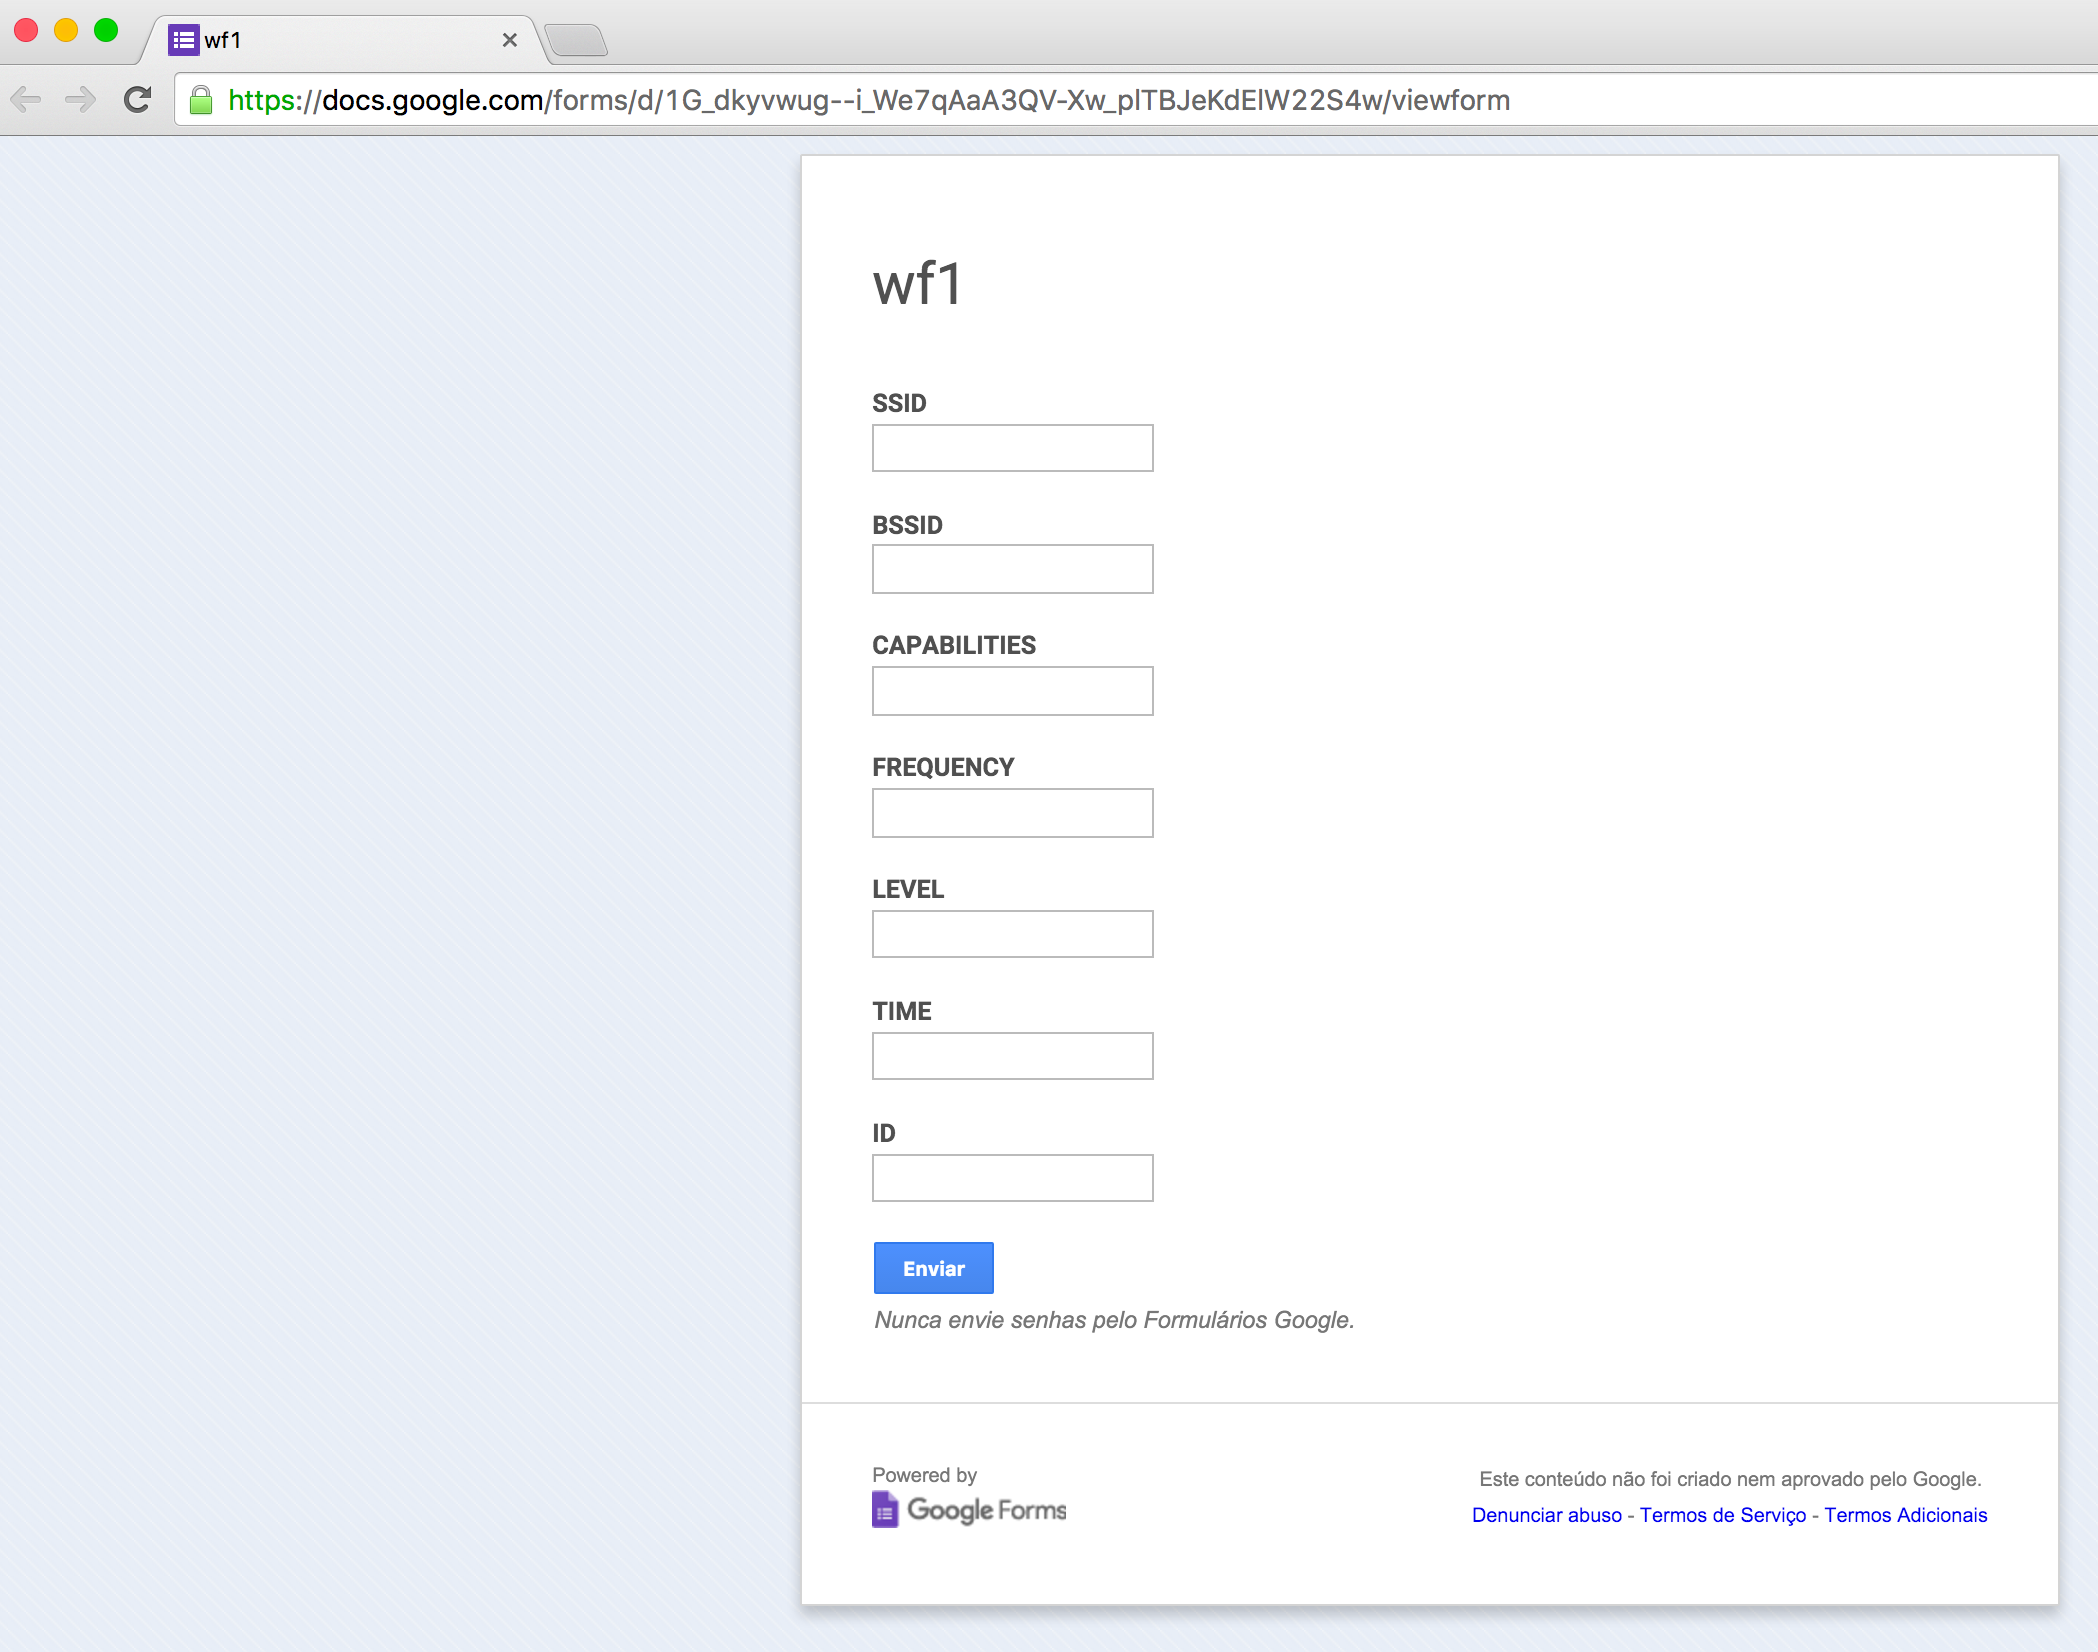
\includegraphics[scale=0.4]{form}
  \caption{Página do formulário utilizado}
\end{figure}


\section{Limpeza dos dados}
Para atender a proposta de limpeza de dados, providenciamos a anonimidade dos usuários contribuintes através da transformação do e-mail coletado pela classe UserEmailFetcher em um hash antes de mandá-lo ao serviço de armazenamento na nuvem.
A seguir temos um exemplo de um registro com as informações \ac{SSID} e ID (identificador do usuário) transformadas em hash. 

\begin{center}
  \begin{tabular}{ l | c | r }
    \hline
    SSID & ID\\ \hline
    8d179f92a46fab285a79929ec51d841a & aa30415a863fa6539cf2e0d741697987 \\ \hline
  \end{tabular}
\end{center}


O código a seguir foi retirado da classe UserEmailFetcher, e é disparado no momento em que estão sendo feitas as requisições POST no formulário do Google Docs. Podemos reparar que na linha 16 é retornado o hash do e-mail de conta Google do usuário, a qual utilizamos como identificador do usuário contribuinte. 



\begin{lstlisting}
	public class UserEmailFetcher
{
  private static Account getAccount(AccountManager paramAccountManager)
  {
    Account[] arrayOfAccount = paramAccountManager.getAccountsByType("com.google");
    if (arrayOfAccount.length > 0)
      return arrayOfAccount[0];
    return null;
  }

  static String getEmail(Context paramContext)
  {
    Account localAccount = getAccount(AccountManager.get(paramContext));
    if (localAccount == null)
      return null;
    return localAccount.name.hashCode().toString();
  }
}
\end{lstlisting}


\chapter{Resultados}
\section{Dados Coletados}
Após divulgação do trabalho para amigos e comunidade, obtivemos mais de 45 mil registros de redes coletadas em um período de aproximadamente um mês. Compilamos os dados com apenas 5 usuários, os quais foram mais colaborativos em questão de quantidade e consideramos o suficiente para analisar os dados.

Importante ressaltar também que a proposta da limpeza de dados, a qual trata os usuários contribuintes com anonimidade, não foi aplicado na coleta dos dados para este trabalho, pelo fato desse paradigma ser aplicado apenas na coleta de dados que visa a contribuição de informações reais para a comunidade.

Com os dados coletados e separados por colaborador compilados em uma planilha, conseguimos o suficiente para realizar algumas análises sobre as informações adquiridas.  Tais análises, serão exibidas na próxima seção.

\section{Análise}
Por se tratar de uma quantidade grande de dados coletados, poderíamos ter realizado diversas análises com propósitos diferentes, mas escolhemos algumas que mais relacionam com o propósito deste trabalho. Por exemplo, na Análise 1, a qual não tratamos de forma anônima para permitir maior insight sobre os resultados, consideramos que a rede ALGARTELECOMVISITANTES seja a do local de trabalho, e a rede ``Lar Doce Lar'' seja a de sua residência, tendo assim um cenário onde o usuário se locomoveu de um local para outro no dia 30/07/2014, e seu dispositivo android coletou e armazenou as informações das redes sem fio ao seu alcance.


Observamos que além das redes citadas acima, o usuário identificado por godinhopatrick@gmail.com visualizou outras 12 redes, isso pode indicar que durante um trajeto que durou aproximadamente 24 minutos, poucas redes foram alcançadas. Tal informação nos leva a concluir que provavelmente o usuário do dispositivo utiliza de um caminho afastado da zona residencial, onde poucas redes foram capturadas, ou a velocidade que estava percorrendo o caminho era alta. 
 
Já na Análise 2, a qual foi tratada com anonimidade, possui redes coletadas no dia 30/07. Consideramos que a rede capturada em seu local de trabalho seja a UFU-Portal e em sua residência a "nao e sua", e tivemos um percurso com mais redes coletadas em um intervalo de tempo semelhante com a análise apresentada na Análise 1. Podemos afirmar então que o usuário da Análise 2 percorreu por um caminho com mais redes sem fio, ou que estava em baixa velocidade permitindo maior frequência de varredura das redes ao redor. Segundo o responsável pelo dispositivo que coletou essas redes, o trajeto é normalmente percorrido a pé.

O conhecimento prévio dos padrões de mobilidade dos usuários destacados nos resultados foi fundamental para a conclusão das análises acima, pois assim consideramos alguns valores tais como locais de trabalho, horário de descanso, dentre outros.

Para considerarmos que um local é o trabalho do usuário e outro é a residência, analisamos a repetição da rede coletada em um determinado intervalo de horário, por exemplo, se no horário comercial um conjunto de redes X é frequentemente capturado, pode-se afirmar que essa localização provavelmente é onde o dono do dispositivo trabalha. No caso da primeira análise apresentada, onde o ID se dá por godinhopatrick@gmail.com, as redes são frequentes e repetitivas durante o período das 09:00 até por volta de 18:00, onde começa uma variação na coleta das redes, o que nos leva a entender que o usuário está se locomovendo.




\small
\setlength\tabcolsep{2pt}
\begin{center}
\begin{longtable}{|c|c|c|c|}

\hline
\textbf{SSID} & \textbf{Capturada em}  & \textbf{ID} \\
\hline
\endfirsthead
\multicolumn{4}{c}%
{\tablename\ \thetable\ -- \textit{Continuação da página anterior}} \\
\hline
\textbf{SSID} & \textbf{Capturada em}  & \textbf{ID} \\
\hline
\endhead
\hline \multicolumn{4}{r}{\textit{Continua na próxima página}} \\
\endfoot
\hline
\endlastfoot
ALGARTELECOM\_VISITANTES  & 00:1f:ca:5f:12:73 & 30/07/2014 06:04:41 & godinhopatrick@gmail.com \\
Invicta                   & 28:10:7b:3c:31:84 & 30/07/2014 06:04:41 & godinhopatrick@gmail.com \\
Maurilio                  & 10:fe:ed:c8:ab:e6 & 30/07/2014 06:04:41 & godinhopatrick@gmail.com \\
Tudo vidros               & c8:d7:19:eb:f6:c7 & 30/07/2014 06:04:41 & godinhopatrick@gmail.com \\
b0c76a                    & 54:be:f7:70:75:4b & 30/07/2014 06:04:41 & godinhopatrick@gmail.com \\
PREMIUMHFC                & bc:f6:85:41:b3:b0 & 30/07/2014 06:04:41 & godinhopatrick@gmail.com \\
CTBC                      & 9c:d6:43:7a:fd:e3 & 30/07/2014 06:04:41 & godinhopatrick@gmail.com \\
Tudo vidros               & c8:d7:19:eb:f6:c7 & 30/07/2014 06:04:41 & godinhopatrick@gmail.com \\
HP-Print-4C-LaserJet 1102 & f4:b7:e2:3c:67:4c & 30/07/2014 06:04:41 & godinhopatrick@gmail.com \\
Tudo vidros               & c8:d7:19:eb:f6:c7 & 30/07/2014 06:04:41 & godinhopatrick@gmail.com \\
CTBC                      & 9c:d6:43:7a:fd:e3 & 30/07/2014 06:04:41 & godinhopatrick@gmail.com \\
Invicta                   & 28:10:7b:3c:31:84 & 30/07/2014 06:04:41 & godinhopatrick@gmail.com \\
ALGARTELECOM\_VISITANTES  & 00:1f:ca:5f:12:73 & 30/07/2014 06:04:41 & godinhopatrick@gmail.com \\
SPEED\_STM2               & 00:0c:42:26:73:39 & 30/07/2014 06:16:03 & godinhopatrick@gmail.com \\
SPEED\_STM2               & 00:0c:42:26:73:39 & 30/07/2014 06:16:03 & godinhopatrick@gmail.com \\
HM2 - FONE: 3084-9493     & 00:80:48:73:fb:db & 30/07/2014 06:23:01 & godinhopatrick@gmail.com \\
HM2 - FONE: 3084-9493     & 00:80:48:73:fb:db & 30/07/2014 06:23:01 & godinhopatrick@gmail.com \\
CTBC                      & 9c:d6:43:7a:bc:0b & 30/07/2014 06:25:45 & godinhopatrick@gmail.com \\
Amanda                    & c0:a0:bb:0f:68:de & 30/07/2014 06:25:45 & godinhopatrick@gmail.com \\
CTBC                      & 9c:d6:43:7a:bc:0b & 30/07/2014 06:25:45 & godinhopatrick@gmail.com \\
Amanda                    & c0:a0:bb:0f:68:de & 30/07/2014 06:25:45 & godinhopatrick@gmail.com \\
Lar Doce Lar              & c0:a0:bb:0e:fa:1e & 30/07/2014 06:28:28 & godinhopatrick@gmail.com \\

\caption{Análise 1}
\centering
\label{Análise 1}
\end{longtable}
\end{center}

\small
\setlength\tabcolsep{2pt}
\begin{center}
\begin{longtable}{|c|c|c|c|c|c|}

\hline
\textbf{SSID} & \textbf{Capturada em}  & \textbf{ID} \\
\hline
\endfirsthead
\multicolumn{4}{c}%
{\tablename\ \thetable\ -- \textit{Continuação da página anterior}} \\
\hline
\textbf{SSID} &  \textbf{Capturada em}  & \textbf{ID} \\
\hline
\endhead
\hline \multicolumn{4}{r}{\textit{Continua na próxima página}} \\
\endfoot
\hline
\caption{Análise 2}
\centering
\label{Análise 2}
\endlastfoot
8d179f92a46fab285a79929ec51d841a & 04/08/2014 05:36:47 & aa30415a863fa6539cf2e0d741697987 \\
8d179f92a46fab285a79929ec51d841a & 04/08/2014 05:36:47 & aa30415a863fa6539cf2e0d741697987 \\
2a7b17a6dd1619a6118f9a8970a8d72b & 04/08/2014 05:36:47 & aa30415a863fa6539cf2e0d741697987 \\
cf6f83af9786671aff636f989852dfe6 & 04/08/2014 05:36:47 & aa30415a863fa6539cf2e0d741697987 \\
8d179f92a46fab285a79929ec51d841a & 04/08/2014 05:36:47 & aa30415a863fa6539cf2e0d741697987 \\
8d179f92a46fab285a79929ec51d841a & 04/08/2014 05:36:47 & aa30415a863fa6539cf2e0d741697987 \\
f30b73d85c69929a5ad6b6d8674aec07 & 04/08/2014 05:36:47 & aa30415a863fa6539cf2e0d741697987 \\
f30b73d85c69929a5ad6b6d8674aec07 & 04/08/2014 05:36:47 & aa30415a863fa6539cf2e0d741697987 \\
b35473767951e29af6bcbdb3aeab94b4 & 04/08/2014 05:45:07 & aa30415a863fa6539cf2e0d741697987 \\
481118ba53b66c5a98d671197054f356 & 04/08/2014 05:45:07 & aa30415a863fa6539cf2e0d741697987 \\
e22fef1f99beaf5788a7b19ac4bffbd1 & 04/08/2014 05:45:07 & aa30415a863fa6539cf2e0d741697987 \\
dcc787b7af1cb9930719dd1f655ebe17 & 04/08/2014 05:45:07 & aa30415a863fa6539cf2e0d741697987 \\
3f5b228294da3490f8b50c459f3f6c87 & 04/08/2014 05:45:07 & aa30415a863fa6539cf2e0d741697987 \\
7f8fa5b29b6dcd1351c92060e8ff9be6 & 04/08/2014 05:45:07 & aa30415a863fa6539cf2e0d741697987 \\
0598065943969ba7156012ea1f856c8a & 04/08/2014 05:45:07 & aa30415a863fa6539cf2e0d741697987 \\
86ebda563945011ee51ed82aa34a16be & 04/08/2014 05:45:07 & aa30415a863fa6539cf2e0d741697987 \\
b0d9e0fb84a27d0645ff7c71cd9f0f8f & 04/08/2014 05:45:07 & aa30415a863fa6539cf2e0d741697987 \\
f54ef483607ec18bd06f55beab2a9a03 & 04/08/2014 05:45:07 & aa30415a863fa6539cf2e0d741697987 \\
365c14d9a42d8d47e575ed5dc688a06e & 04/08/2014 05:45:07 & aa30415a863fa6539cf2e0d741697987 \\
3e443977126ec80b11db0cae5a9bdccc & 04/08/2014 05:45:07 & aa30415a863fa6539cf2e0d741697987 \\
97f012aa3ead49fc98583d282ca71d49 & 04/08/2014 05:45:07 & aa30415a863fa6539cf2e0d741697987 \\
282301c0f75d5c985999e60ab73f7e23 & 04/08/2014 05:45:07 & aa30415a863fa6539cf2e0d741697987 \\
4b96d5c1ff312eea069ddc760794963d & 04/08/2014 05:45:07 & aa30415a863fa6539cf2e0d741697987 \\
9f3b7f3d66fb537342e2993c2574b02b & 04/08/2014 05:45:07 & aa30415a863fa6539cf2e0d741697987 \\
6b2ef1b90924ba3c786ea2f6a98a046e & 04/08/2014 05:45:07 & aa30415a863fa6539cf2e0d741697987 \\
59422c6d30247893a2c77777d90b6c30 & 04/08/2014 05:45:07 & aa30415a863fa6539cf2e0d741697987 \\
a50bd3499ef74cead938f7338df2709b & 04/08/2014 05:49:33 & aa30415a863fa6539cf2e0d741697987 \\
591d9b34d1f48055596eb6b7455af526 & 04/08/2014 05:49:33 & aa30415a863fa6539cf2e0d741697987 \\
fa3835a18d4dbb8093bedeaf6ff0bd21 & 04/08/2014 05:49:33 & aa30415a863fa6539cf2e0d741697987 \\
6317a2a78153fe49b9e7b42ab1870759 & 04/08/2014 05:49:33 & aa30415a863fa6539cf2e0d741697987 \\
82cfc75e5d5a2ca07073babc666e7537 & 04/08/2014 05:49:33 & aa30415a863fa6539cf2e0d741697987 \\
0c845f83efa0c9869933c5ca8f5b07bb & 04/08/2014 05:49:33 & aa30415a863fa6539cf2e0d741697987 \\
c8bbe67803085b9e51b69b6d6cff821c & 04/08/2014 05:49:33 & aa30415a863fa6539cf2e0d741697987 \\
5bc1b8af009e072d5ef1d18d3fe0b961 & 04/08/2014 05:49:33 & aa30415a863fa6539cf2e0d741697987 \\
8b0131121330dc9990e704c62e6cf5c2 & 04/08/2014 05:49:33 & aa30415a863fa6539cf2e0d741697987 \\
ac4b5d776485a84bd0a58dc2af669667 & 04/08/2014 05:49:33 & aa30415a863fa6539cf2e0d741697987 \\
d49fab26ac2dfc1970ae462229264f35 & 04/08/2014 05:49:33 & aa30415a863fa6539cf2e0d741697987 \\
695d5cf06094d7e2e93c4d347fadaf36 & 04/08/2014 05:49:33 & aa30415a863fa6539cf2e0d741697987 \\
e98c5ddd42ada2c6fec5aff29e4631f2 & 04/08/2014 05:49:33 & aa30415a863fa6539cf2e0d741697987 \\
54dcc7d6ea31638a26b17078fc8ea2d8 & 04/08/2014 05:54:11 & aa30415a863fa6539cf2e0d741697987 \\
ea1dd8b9142f0bc51852cf0676a643dd & 04/08/2014 05:54:11 & aa30415a863fa6539cf2e0d741697987 \\
1f44c499f4e7259b28a9a6504c0ba5c0 & 04/08/2014 05:54:11 & aa30415a863fa6539cf2e0d741697987 \\
f1446884609e12fc723f383b6e88ad7b & 04/08/2014 05:54:11 & aa30415a863fa6539cf2e0d741697987 \\
017add08f76ecc11b0c719c3d39a3d0e & 04/08/2014 05:54:11 & aa30415a863fa6539cf2e0d741697987 \\
3c69bdf979acbffd0749803659fc8cef & 04/08/2014 05:54:11 & aa30415a863fa6539cf2e0d741697987 \\
eab9aadba9775e4d16331f4710e6dbd8 & 04/08/2014 05:54:11 & aa30415a863fa6539cf2e0d741697987 \\
a214a35493406ea8ad965c3822fdaec4 & 04/08/2014 05:54:11 & aa30415a863fa6539cf2e0d741697987 \\
1c91ef773c27b7777f9bcee616eb7622 & 04/08/2014 05:54:11 & aa30415a863fa6539cf2e0d741697987 \\
e05747eda27888a8db3fca1f1e981757 & 04/08/2014 05:54:11 & aa30415a863fa6539cf2e0d741697987 \\
f1446884609e12fc723f383b6e88ad7b & 04/08/2014 05:58:02 & aa30415a863fa6539cf2e0d741697987 \\
017add08f76ecc11b0c719c3d39a3d0e & 04/08/2014 05:58:02 & aa30415a863fa6539cf2e0d741697987 \\
1c91ef773c27b7777f9bcee616eb7622 & 04/08/2014 05:58:02 & aa30415a863fa6539cf2e0d741697987 \\
e05747eda27888a8db3fca1f1e981757 & 04/08/2014 05:58:02 & aa30415a863fa6539cf2e0d741697987 \\
9854f58dee424e44ae3f222fc8faf310 & 04/08/2014 05:58:02 & aa30415a863fa6539cf2e0d741697987 \\
a214a35493406ea8ad965c3822fdaec4 & 04/08/2014 05:58:02 & aa30415a863fa6539cf2e0d741697987 \\
3c69bdf979acbffd0749803659fc8cef & 04/08/2014 05:58:02 & aa30415a863fa6539cf2e0d741697987 \\
1f44c499f4e7259b28a9a6504c0ba5c0 & 04/08/2014 05:58:02 & aa30415a863fa6539cf2e0d741697987 \\
a214a35493406ea8ad965c3822fdaec4 & 04/08/2014 05:58:02 & aa30415a863fa6539cf2e0d741697987 \\
304d60913d528570624670b9523f9f1c & 04/08/2014 05:58:02 & aa30415a863fa6539cf2e0d741697987 \\
54dcc7d6ea31638a26b17078fc8ea2d8 & 04/08/2014 06:04:15 & aa30415a863fa6539cf2e0d741697987 \\
b8ca0faeb96bb246a93f1ec705904a98 & 04/08/2014 06:04:15 & aa30415a863fa6539cf2e0d741697987 \\
3c69bdf979acbffd0749803659fc8cef & 04/08/2014 06:04:15 & aa30415a863fa6539cf2e0d741697987 \\
c91bac5fdd1df5ef0480a1cb86052109 & 04/08/2014 06:04:15 & aa30415a863fa6539cf2e0d741697987 \\
37c621181b9c749581bced45f0546441 & 04/08/2014 06:04:15 & aa30415a863fa6539cf2e0d741697987 \\
09fdc52c75480000a14307d2ae99c3ba & 04/08/2014 06:04:15 & aa30415a863fa6539cf2e0d741697987 \\
fb6d70a2d9f2e57507dd5f0126d8f69f & 04/08/2014 06:04:15 & aa30415a863fa6539cf2e0d741697987 \\
5a422641ca0a57a1397ca32c3a2ed5fe & 04/08/2014 06:04:15 & aa30415a863fa6539cf2e0d741697987 \\
bd42313705de24c3cc797db9feb9db68 & 04/08/2014 06:04:15 & aa30415a863fa6539cf2e0d741697987 \\
a214a35493406ea8ad965c3822fdaec4 & 04/08/2014 06:04:15 & aa30415a863fa6539cf2e0d741697987 \\
eba296a8391167ce48a94dea70eb5b0b & 04/08/2014 06:09:44 & aa30415a863fa6539cf2e0d741697987 \\
2816b5665ca0d9db7a6a0816b88324f7 & 04/08/2014 06:09:44 & aa30415a863fa6539cf2e0d741697987 \\
b6a793033f0fd4483d30ef37e3d5b058 & 04/08/2014 06:09:44 & aa30415a863fa6539cf2e0d741697987 \\
5bc1b8af009e072d5ef1d18d3fe0b961 & 04/08/2014 06:09:44 & aa30415a863fa6539cf2e0d741697987 \\
c709be5445f65fea03e6f82a924a5463 & 04/08/2014 06:09:44 & aa30415a863fa6539cf2e0d741697987 \\
f3de1da2923631f028a6b572bb61f86d & 04/08/2014 06:09:44 & aa30415a863fa6539cf2e0d741697987 \\
32c7b4d0b73d86e9fa9b5e0ea7886725 & 04/08/2014 06:09:44 & aa30415a863fa6539cf2e0d741697987 \\
f30ebc9e686cde3a3d476a53c3405bf4 & 04/08/2014 06:09:44 & aa30415a863fa6539cf2e0d741697987 \\
60f8d2b10615467782bffa56886e7e93 & 04/08/2014 06:09:44 & aa30415a863fa6539cf2e0d741697987 \\
ac4b5d776485a84bd0a58dc2af669667 & 04/08/2014 06:09:44 & aa30415a863fa6539cf2e0d741697987 \\
a01df980e93c383e70a030e9df196ed4 & 04/08/2014 06:09:44 & aa30415a863fa6539cf2e0d741697987 \\
c8f65e3e220278c7000f9330cb9f02b9 & 04/08/2014 06:09:44 & aa30415a863fa6539cf2e0d741697987 \\
a09b70da3de1d3c861c392d804d0d63d & 04/08/2014 06:09:44 & aa30415a863fa6539cf2e0d741697987 \\
e61851dde94d0a25c011b19d4804a986 & 04/08/2014 06:09:44 & aa30415a863fa6539cf2e0d741697987 \\
 & 04/08/2014 06:09:44 & aa30415a863fa6539cf2e0d741697987 \\
b4326946e1986fe9b5e979b82744d3bf & 04/08/2014 06:09:44 & aa30415a863fa6539cf2e0d741697987 \\
f1aab358cebf94d40cac149f9c894f2f & 04/08/2014 06:09:44 & aa30415a863fa6539cf2e0d741697987 \\
cb4b7003fae5898afe4faa0e844ccaca & 04/08/2014 06:09:44 & aa30415a863fa6539cf2e0d741697987 \\
7b90375d81759fc3b6e13df1569bad30 & 04/08/2014 06:09:44 & aa30415a863fa6539cf2e0d741697987 \\
3e6a09208e022fcddf43ac30460916f0 & 04/08/2014 06:09:44 & aa30415a863fa6539cf2e0d741697987 \\
890d4940c42e231dd55d98d04404b588 & 04/08/2014 06:09:44 & aa30415a863fa6539cf2e0d741697987 \\
8a3912022f071a3b2dd71146a460ba46 & 04/08/2014 06:09:44 & aa30415a863fa6539cf2e0d741697987 \\
ce7eede2166e6b6193aab0c1b4e20c40 & 04/08/2014 06:09:44 & aa30415a863fa6539cf2e0d741697987 \\
f5e5714978904472691feaed59b1eef9 & 04/08/2014 06:09:44 & aa30415a863fa6539cf2e0d741697987 \\
0f125204dd3e8b55dcc0acf3f11b665a & 04/08/2014 06:09:44 & aa30415a863fa6539cf2e0d741697987 \\
9d910c8bf395fce35216f0f4fa85432e & 04/08/2014 06:09:44 & aa30415a863fa6539cf2e0d741697987 \\
f95d2d1f4f6dd82d81a7dbc61131bf01 & 04/08/2014 06:09:44 & aa30415a863fa6539cf2e0d741697987 \\
4a24f63118ba52985ee3a81bebf726af & 04/08/2014 06:09:44 & aa30415a863fa6539cf2e0d741697987 \\
f6b60e5ca673f596a2f2f320426aaac4 & 04/08/2014 06:09:44 & aa30415a863fa6539cf2e0d741697987 \\
c03dfe946e14ad8a533c5b31fceee8f4 & 04/08/2014 06:12:56 & aa30415a863fa6539cf2e0d741697987 \\
19f07cd585213b7ee536d220dd5e05d8 & 04/08/2014 06:12:56 & aa30415a863fa6539cf2e0d741697987 \\
17e0e126a99a3d00707cb0325aeb19e5 & 04/08/2014 06:12:56 & aa30415a863fa6539cf2e0d741697987 \\
4768a8e7987fa0b08f8f1e89771d537c & 04/08/2014 06:12:56 & aa30415a863fa6539cf2e0d741697987 \\
d11a0cdb886402501984e622b9f9ea91 & 04/08/2014 06:12:56 & aa30415a863fa6539cf2e0d741697987 \\
3da9b84ddf62db911fdad28e92dddb40 & 04/08/2014 06:12:56 & aa30415a863fa6539cf2e0d741697987 \\
bdd53871142b53476f42934dd959c3c2 & 04/08/2014 06:12:56 & aa30415a863fa6539cf2e0d741697987 \\
2422427f25a06de54ee468174e97ebef & 04/08/2014 06:12:56 & aa30415a863fa6539cf2e0d741697987 \\
f2cb32166f77f33e80311be40c97466e & 04/08/2014 06:12:56 & aa30415a863fa6539cf2e0d741697987 \\
382aab5ef70b2b3c791bc42698cd6bfc & 04/08/2014 06:12:56 & aa30415a863fa6539cf2e0d741697987 \\
266d530043c3258b02f3e35a70191d35 & 04/08/2014 06:12:56 & aa30415a863fa6539cf2e0d741697987 \\
9097ab90f86c8c35103a826720359f4a & 04/08/2014 06:12:56 & aa30415a863fa6539cf2e0d741697987 \\
4768a8e7987fa0b08f8f1e89771d537c & 04/08/2014 06:12:56 & aa30415a863fa6539cf2e0d741697987 \\
e4963bf7fbea0240c7c41753fd752b26 & 04/08/2014 06:12:56 & aa30415a863fa6539cf2e0d741697987 \\
ecf12bac029e5a5d2054320574022f5f & 04/08/2014 06:12:56 & aa30415a863fa6539cf2e0d741697987 \\
640f527ef3c0c140886298349f24573b & 04/08/2014 06:12:56 & aa30415a863fa6539cf2e0d741697987 \\
45b5b81c8e2420a7aac2ff1c475711f6 & 04/08/2014 06:12:56 & aa30415a863fa6539cf2e0d741697987 \\
d97cbb5fdec044e0b246e41405efc759 & 04/08/2014 06:12:56 & aa30415a863fa6539cf2e0d741697987 \\
c80a3eaff0aa4d1d86e2f3afbc45a355 & 04/08/2014 06:12:56 & aa30415a863fa6539cf2e0d741697987 \\
60a46f8d9050564cb1f40de9daa92c8a & 04/08/2014 06:12:56 & aa30415a863fa6539cf2e0d741697987 \\
a9be98e01836b20aba0e32aeb61285f5 & 04/08/2014 06:12:56 & aa30415a863fa6539cf2e0d741697987 \\
4b6152705aefea15a3423257e7f98b2b & 04/08/2014 06:12:56 & aa30415a863fa6539cf2e0d741697987 \\
c3556d9438b0c421cea89bc436f403c2 & 04/08/2014 06:12:56 & aa30415a863fa6539cf2e0d741697987 \\
4768a8e7987fa0b08f8f1e89771d537c & 04/08/2014 06:17:05 & aa30415a863fa6539cf2e0d741697987 \\
c80a3eaff0aa4d1d86e2f3afbc45a355 & 04/08/2014 06:17:05 & aa30415a863fa6539cf2e0d741697987 \\
640f527ef3c0c140886298349f24573b & 04/08/2014 06:17:05 & aa30415a863fa6539cf2e0d741697987 \\
a9be98e01836b20aba0e32aeb61285f5 & 04/08/2014 06:17:05 & aa30415a863fa6539cf2e0d741697987 \\
4b6152705aefea15a3423257e7f98b2b & 04/08/2014 06:17:05 & aa30415a863fa6539cf2e0d741697987 \\
c3556d9438b0c421cea89bc436f403c2 & 04/08/2014 06:17:05 & aa30415a863fa6539cf2e0d741697987 \\
91d6092214818341b2f55287b1bc90bc & 04/08/2014 06:17:05 & aa30415a863fa6539cf2e0d741697987 \\
623cedfd93c052ee5787bbb9d11dd742 & 04/08/2014 06:17:06 & aa30415a863fa6539cf2e0d741697987 \\
4768a8e7987fa0b08f8f1e89771d537c & 04/08/2014 06:18:06 & aa30415a863fa6539cf2e0d741697987 \\
c80a3eaff0aa4d1d86e2f3afbc45a355 & 04/08/2014 06:18:06 & aa30415a863fa6539cf2e0d741697987 \\
640f527ef3c0c140886298349f24573b & 04/08/2014 06:18:06 & aa30415a863fa6539cf2e0d741697987 \\
\end{longtable}
\end{center}

Outro cenário interessante de se analisar é a quantidade de vezes que uma rede foi coletada em um certo intervalo de tempo. Por exemplo na Figura 9, que ilustra a data de 28/05/2014 em um intervalo de tempo entre 00:00 e 18:20,  onde é exibido o nome da rede bem como a quantidade que ela foi coletada pelo aplicativo. 

\begin{figure}[hbt]
  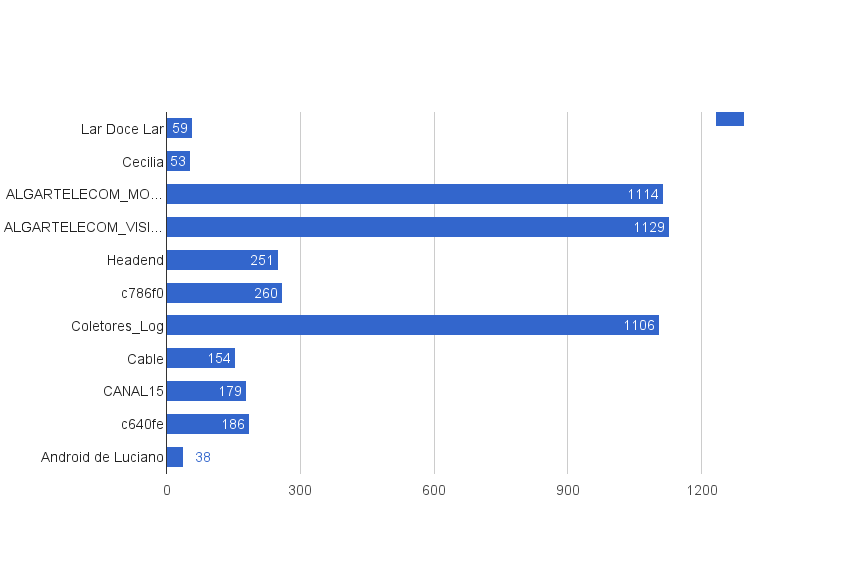
\includegraphics[scale=0.4]{analise3}
  \caption{Análise 3 - Redes coletadas no dia 28/05/2014 - 00:00 as 18:20}
\end{figure}


Para essa análise, foram filtradas as redes que foram coletadas mais que 30 vezes, para eliminarmos as que para esse cenário não nos interessa. Concluímos com esse gráfico que mesmo o usuário permanecendo a mesma quantidade de tempo no alcance das redes Lar Doce Lar, local onde reside,  e as redes ALGARTELECOM, local onde trabalha, as redes sem fio do trabalho foram mais frequentes na coleta, isso se deu pela quantidade de pontos fornecedores, como replicadores e roteadores, (com MAC Address diferentes) de uma mesma rede, onde para cada uma alcançada é criado um novo registro na base de dados do dispositivo. 

Identificamos também a necessidade de descobrir se o padrão de coleta das redes sem fio se repetiam todos os dias, ou seja, inclusive sábados e domingos. Concluímos que não, pois teve alteração das redes sem fio nos fins de semana,  como por exemplo na Tabela 3 abaixo, onde ilustra as redes coletadas pelo mesmo usuário da Figura 9, em um sábado.

\small
\setlength\tabcolsep{2pt}
\begin{center}
\begin{longtable}{|c|c|c|c|c|c|}

\hline
\textbf{SSID} & \textbf{Capturada em}  & \textbf{ID} \\
\hline
\endfirsthead
\multicolumn{4}{c}%
{\tablename\ \thetable\ -- \textit{Continuação da página anterior}} \\
\hline
\textbf{SSID} &  \textbf{Capturada em}  & \textbf{ID} \\
\hline
\endhead
\hline \multicolumn{4}{r}{\textit{Continua na próxima página}} \\
\endfoot
\hline
\caption{Análise 4}
\centering
\label{Análise 4}
\endlastfoot
Rede Hoteis Prive                 & 09/08/2014 07:40:10 & godinhopatrick@gmail.com \\
Boulevard\_recepcao               & 09/08/2014 07:40:10 & godinhopatrick@gmail.com \\
Boulevard-B                       & 09/08/2014 07:40:10 & godinhopatrick@gmail.com \\
Rede Prive Diversao               & 09/08/2014 07:44:19 & godinhopatrick@gmail.com \\
Rede Prive Diversao               & 09/08/2014 07:40:10 & godinhopatrick@gmail.com \\
Boulevard-A                       & 09/08/2014 07:40:10 & godinhopatrick@gmail.com \\
Recepcao\_Lobby-TDM               & 09/08/2014 07:40:10 & godinhopatrick@gmail.com \\
Rede Hoteis Prive                 & 09/08/2014 07:40:10 & godinhopatrick@gmail.com \\
CALDAS\_DIGITAL\_III              & 09/08/2014 07:40:10 & godinhopatrick@gmail.com \\
Prive\_TDM-B                      & 09/08/2014 07:40:10 & godinhopatrick@gmail.com \\
Prive\_TDM-A                      & 09/08/2014 07:40:10 & godinhopatrick@gmail.com \\
CHOPERIA\_BOULEVARD               & 09/08/2014 07:40:10 & godinhopatrick@gmail.com \\
Prive\_Area\_de\_Lazer            & 09/08/2014 07:40:10 & godinhopatrick@gmail.com \\
Prive\_TDM-C                      & 09/08/2014 07:40:10 & godinhopatrick@gmail.com \\
Boulevard-B                       & 09/08/2014 07:40:10 & godinhopatrick@gmail.com \\
Rede Prive Diversao               & 09/08/2014 07:47:18 & godinhopatrick@gmail.com \\
ROYAL-B5                          & 09/08/2014 07:47:18 & godinhopatrick@gmail.com \\
ROYAL-B4                          & 09/08/2014 07:47:18 & godinhopatrick@gmail.com \\
Boulevard-A                       & 09/08/2014 07:47:18 & godinhopatrick@gmail.com \\
Recepcao\_Lobby-TDM               & 09/08/2014 07:47:18 & godinhopatrick@gmail.com \\
Prive\_Area\_de\_Lazer            & 09/08/2014 07:47:18 & godinhopatrick@gmail.com \\
CALDAS\_DIGITAL\_III              & 09/08/2014 07:47:18 & godinhopatrick@gmail.com \\
Prive\_TDM-B                      & 09/08/2014 07:47:18 & godinhopatrick@gmail.com \\
Rede Hoteis Prive                 & 09/08/2014 07:47:18 & godinhopatrick@gmail.com \\
Prive\_TDM-C                      & 09/08/2014 07:47:18 & godinhopatrick@gmail.com \\
lanteca\_varandas\_M5\_II         & 09/08/2014 07:47:19 & godinhopatrick@gmail.com \\
Boulevard-C                       & 09/08/2014 07:47:19 & godinhopatrick@gmail.com \\
Boulevard-A                       & 09/08/2014 07:47:19 & godinhopatrick@gmail.com \\
ROYAL-B3                          & 09/08/2014 07:47:19 & godinhopatrick@gmail.com \\
LUCIMAR-MARCOS                    & 09/08/2014 07:47:19 & godinhopatrick@gmail.com \\
Afpichelli                        & 09/08/2014 07:47:19 & godinhopatrick@gmail.com \\
Boulevard-B                       & 09/08/2014 07:47:19 & godinhopatrick@gmail.com \\
Boulevard-B                       & 09/08/2014 07:47:19 & godinhopatrick@gmail.com \\
WIFI\_ROYAL                       & 09/08/2014 07:47:19 & godinhopatrick@gmail.com \\
DEXLINK-RTWL15F1                  & 09/08/2014 07:47:19 & godinhopatrick@gmail.com \\
Boulevard-C                       & 09/08/2014 07:47:19 & godinhopatrick@gmail.com \\
Rede Prive Diversao               & 09/08/2014 07:48:18 & godinhopatrick@gmail.com \\
ROYAL-B4                          & 09/08/2014 07:48:18 & godinhopatrick@gmail.com \\
Boulevard-A                       & 09/08/2014 07:48:18 & godinhopatrick@gmail.com \\
Recepcao\_Lobby-TDM               & 09/08/2014 07:48:18 & godinhopatrick@gmail.com \\
LUCIMAR-MARCOS                    & 09/08/2014 07:48:18 & godinhopatrick@gmail.com \\
Boulevard-B                       & 09/08/2014 07:48:18 & godinhopatrick@gmail.com \\
ROYAL-B3                          & 09/08/2014 07:48:18 & godinhopatrick@gmail.com \\
HPPRIMAVERA                       & 09/08/2014 07:48:18 & godinhopatrick@gmail.com \\
ROYAL-B1                          & 09/08/2014 07:48:18 & godinhopatrick@gmail.com \\
Prive\_TDM-B                      & 09/08/2014 07:48:18 & godinhopatrick@gmail.com \\
WIFI\_ROYAL                       & 09/08/2014 07:48:18 & godinhopatrick@gmail.com \\
Prive\_TDM-A                      & 09/08/2014 07:48:18 & godinhopatrick@gmail.com \\
CALDAS\_DIGITAL\_PARQUINHO        & 09/08/2014 07:48:18 & godinhopatrick@gmail.com \\
Prive\_TDM-C                      & 09/08/2014 07:48:18 & godinhopatrick@gmail.com \\
HOTCALDAS\_MC1                    & 09/08/2014 07:48:18 & godinhopatrick@gmail.com \\
HOUSE TECH                        & 09/08/2014 07:49:46 & godinhopatrick@gmail.com \\
LOJA LAGOA                        & 09/08/2014 07:49:46 & godinhopatrick@gmail.com \\
STFCS                             & 09/08/2014 07:49:46 & godinhopatrick@gmail.com \\
HGR                               & 09/08/2014 07:49:46 & godinhopatrick@gmail.com \\
Residencial                       & 09/08/2014 07:49:46 & godinhopatrick@gmail.com \\
EXCLUSIVE                         & 09/08/2014 07:49:46 & godinhopatrick@gmail.com \\
FLAVIA                            & 09/08/2014 07:49:46 & godinhopatrick@gmail.com \\
                                  & 09/08/2014 07:49:46 & godinhopatrick@gmail.com \\
TV RIO PARANAIBA                  & 09/08/2014 07:49:46 & godinhopatrick@gmail.com \\
KITAKAS                           & 09/08/2014 07:49:46 & godinhopatrick@gmail.com \\
Pousada do Galego                 & 09/08/2014 07:49:46 & godinhopatrick@gmail.com \\
CLEAN                             & 09/08/2014 07:49:46 & godinhopatrick@gmail.com \\
Residencial Tropical              & 09/08/2014 07:49:46 & godinhopatrick@gmail.com \\
redesudeste2                      & 09/08/2014 07:49:46 & godinhopatrick@gmail.com \\
Aruba 1                           & 09/08/2014 07:49:46 & godinhopatrick@gmail.com \\
arterara                          & 09/08/2014 07:49:46 & godinhopatrick@gmail.com \\
privediversao                     & 09/08/2014 07:49:46 & godinhopatrick@gmail.com \\
CALDAS\_DIGITAL\_MESTREORLANDO\_I & 09/08/2014 07:53:39 & godinhopatrick@gmail.com \\
AP-24-EBG-S3                      & 09/08/2014 07:53:39 & godinhopatrick@gmail.com \\
ALQUIMIA 01                       & 09/08/2014 07:53:39 & godinhopatrick@gmail.com \\
ATALAIA-WIFI                      & 09/08/2014 07:53:39 & godinhopatrick@gmail.com \\
CONVIDADOS-ATALAIA                & 09/08/2014 07:53:39 & godinhopatrick@gmail.com \\
ATALAIA-WIFI                      & 09/08/2014 07:53:39 & godinhopatrick@gmail.com \\
                                  & 09/08/2014 07:53:39 & godinhopatrick@gmail.com \\
ATALAIA-WIFI                      & 09/08/2014 07:53:39 & godinhopatrick@gmail.com \\
AP-2x2-58-EBG-S1                  & 09/08/2014 07:53:39 & godinhopatrick@gmail.com \\
ATALAIA-WIFI                      & 09/08/2014 07:53:39 & godinhopatrick@gmail.com \\
CONVIDADOS-ATALAIA                & 09/08/2014 07:53:39 & godinhopatrick@gmail.com \\
LOJA VANIA                        & 09/08/2014 07:53:39 & godinhopatrick@gmail.com \\
PapCentral                        & 09/08/2014 07:53:39 & godinhopatrick@gmail.com \\
CONVIDADOS-ATALAIA                & 09/08/2014 07:53:39 & godinhopatrick@gmail.com \\
CONVIDADOS-ATALAIA                & 09/08/2014 07:53:39 & godinhopatrick@gmail.com \\
Papelaria Central                 & 09/08/2014 07:53:39 & godinhopatrick@gmail.com \\
Maria\_Alves                      & 09/08/2014 07:53:39 & godinhopatrick@gmail.com \\
ATALAIA-WIFI                      & 09/08/2014 07:53:39 & godinhopatrick@gmail.com \\
AP-2x2-58-EBG-S4                  & 09/08/2014 07:53:39 & godinhopatrick@gmail.com \\
HOTCALDASARB1                     & 09/08/2014 07:53:39 & godinhopatrick@gmail.com \\
GLOBALNET\_III                    & 09/08/2014 08:25:35 & godinhopatrick@gmail.com \\
Ilton                             & 09/08/2014 08:25:35 & godinhopatrick@gmail.com \\
GLOBALNET\_M5\_I                  & 09/08/2014 08:25:35 & godinhopatrick@gmail.com \\
Italac-4                          & 09/08/2014 08:25:35 & godinhopatrick@gmail.com \\
GLOBALNET\_II                     & 09/08/2014 08:25:35 & godinhopatrick@gmail.com \\
Rogerio                           & 09/08/2014 08:28:17 & godinhopatrick@gmail.com \\
GLOBALNET\_I                      & 09/08/2014 08:28:17 & godinhopatrick@gmail.com \\
pontonet-002                      & 09/08/2014 08:28:17 & godinhopatrick@gmail.com \\
pontonet-001                      & 09/08/2014 08:28:17 & godinhopatrick@gmail.com \\
GLOBALNET\_III                    & 09/08/2014 08:28:17 & godinhopatrick@gmail.com \\
PTP-Minas                         & 09/08/2014 08:42:20 & godinhopatrick@gmail.com \\
pontonet-64-3447-2050             & 09/08/2014 08:42:20 & godinhopatrick@gmail.com \\
Soft5g64                          & 09/08/2014 09:19:07 & godinhopatrick@gmail.com \\
Soft09                            & 09/08/2014 09:19:07 & godinhopatrick@gmail.com \\
altlore                           & 09/08/2014 09:19:07 & godinhopatrick@gmail.com
\end{longtable}
\end{center}

Através da Tabela 3 podemos deduzir pelos nomes das redes, que no dia 09/08/2014, sábado, o usuário foi para Caldas Novas - GO, fugindo assim do padrão das redes que coletava quando estava em sua residência ou no trabalho. Assim concluímos que não podemos garantir que os pontos coletados diariamente se repetem até nos sábados e domingos, mas podemos dizer que existe uma grande probabilidade de se repetir em dias de semana, onde a rotina de vida do usuário o induz a ser repetitivo.


Mais análises são possíveis de ser construídas, porém pela limitação do serviço que utilizamos para armazenar, o Google Docs Sheets, as anteriores foram as escolhidas para demonstrar a importância do nosso protótipo de aplicativo, bem como o que foi, e pode ser produzido através dele.



\chapter{Conclusão}


Com o desenvolvimento desse trabalho, concluímos que existe um potencial enorme em pesquisas no campo de redes móveis, principalmente no trabalho base seguido, o PheroCast. Ficamos satisfeitos com o resultado de ter o protótipo implementado, e mostrar o grande potencial a ser explorado no que se refere às análises dos dados coletados. Também podemos contribuir com a pesquisa de predição da localização de um nó em uma rede móvel, dentre outras pesquisas na comunidade que demandam de dados reais de ``rastros'' como os capturados através do produto final deste trabalho, o aplicativo PheroCast App.


Para trabalhos futuros, pretendemos implementar também a coleta e armazenamento das localizações por GPS, capturadas também pelo dispositivo móvel. Outro ponto a ser implementado futuramente, como mencionado, será a limpeza dos dados para garantir a anonimidade dos contribuintes dos dados.

Para melhorar mais ainda o trabalho, indicamos também um serviço de armazenamento na nuvem com uma base de dados mais robusta, a fim de gerar relatórios mais analíticos, pois o Google Docs, serviço utilizado nesse trabalho, não atende uma grande demanda de dados, visto que com os dados coletados neste trabalho a performance ao operar as planilhas é bem pequena. 

Concluímos também que a arquitetura, implementação e desenvolvimento do aplicativo bem como a produção das análises com os dados produzidos pela utilização do software por algumas pessoas da comunidade, foi consequência da base de conhecimento adquirida durante o curso de Sistemas de Informação da Universidade Federal de Uberlândia, bem como o tempo de pesquisa aplicado nesse trabalho. Tais ações e resultados implicam no sucesso deste trabalho de conclusão de curso.

%\chapter{Revisão Bibliográfica}
%TCC:

%Um ou mais capítulos (por exemplo, se há duas linhas de trabalhos relacionados.


% ----------------------------------------------------------
% ELEMENTOS PÓS-TEXTUAIS
% ----------------------------------------------------------
\postextual


% ----------------------------------------------------------
% Referências bibliográficas
% ----------------------------------------------------------
\nocite{6710069}
\nocite{IBM:Android}

\bibliography{bib}


%% ----------------------------------------------------------
%% Apêndices TCC: só mantenha se for pertinente.
%% ----------------------------------------------------------

% ---
% Inicia os apêndices
% ---


% ----------------------------------------------------------
% Anexos %TCC: so mantenha se pertinente.
% ----------------------------------------------------------

% ---
% Inicia os anexos
% ---
\begin{anexosenv}

% Imprime uma página indicando o início dos anexos
\partanexos

% ---
\chapter{Código fonte}
% 
\section{MainActivity.java}
\begin{lstlisting}
package ufu.tcc.patrick.pherocast;
import android.annotation.SuppressLint;
import android.content.BroadcastReceiver;
import android.content.Context;
import android.content.Intent;
import android.content.IntentFilter;
import android.net.wifi.ScanResult;
import android.net.wifi.WifiManager;
import android.os.Bundle;
import android.os.Handler;
import android.support.v7.app.ActionBarActivity;
import android.widget.TextView;
import android.widget.Toast;

import java.io.PrintStream;
import java.text.SimpleDateFormat;
import java.util.ArrayList;
import java.util.Date;
import java.util.List;
import java.util.Timer;
import java.util.TimerTask;

public class MainActivity extends ActionBarActivity {
	final Handler handler = new Handler();
	boolean scanInitiated;
	TimerTask scanTask;
	Timer t = new Timer();
	TextView text;
	WifiManager wifi;
	boolean wifiOn;
	WifiScanReceiver wifiReciever;
	String[] wifis;
	List<ScanResult> localList = new ArrayList<ScanResult>();

	private String pegarHoraAtual() {
		return new SimpleDateFormat("dd/MM/yyyy hh:mm:ss").format(new Date()); 
	}

	public void getWifiState() {
		System.out.println("passou aqui " + wifi.isWifiEnabled());
		if (!wifi.isWifiEnabled()) {
			wifiOn = false;
			Toast.makeText(getApplicationContext(),
					"Wifi desativado, estamos ativando...", 1).show();
			wifi.setWifiEnabled(true);
			return;
		}
		wifiOn = true;
	}

	public void onBackPressed() {
		moveTaskToBack(true);
	}

	protected void onCreate(Bundle paramBundle) {
		super.onCreate(paramBundle);
		setContentView(2130903064);
		wifi = ((WifiManager) getSystemService("wifi"));
		wifiReciever = new WifiScanReceiver();
		scanTask = new TimerTask() {
			public void run() {
				handler.post(new Runnable() {
					public void run() {
						getWifiState();
						registerReceiver(wifiReciever, new IntentFilter(
								"android.net.wifi.SCAN_RESULTS"));
						scanInitiated = true;
						wifi.startScan();
					}
				});
			}
		};
		t.schedule(scanTask, 300L, 60000L);
	}

	class WifiScanReceiver extends BroadcastReceiver {
		WifiScanReceiver() {
		}

		@SuppressLint({ "UseValueOf", "NewApi" })
		public void onReceive(Context paramContext, Intent paramIntent) {

			NetworkPointDAO localNetworkPointDAO = NetworkPointDAO
					.getInstance(getBaseContext());
			if (scanInitiated) {
				localList = wifi.getScanResults();
				wifis = new String[localList.size()];

			}
			for (int i = 0;; i++) {
				if (i >= localList.size()) {
					scanInitiated = false;
					System.out.println(wifiOn);
					if (!wifiOn)
						wifi.setWifiEnabled(false);
					unregisterReceiver(this);
					return;
				}
				wifis[i] = (((ScanResult) localList.get(i)).SSID + ", "
						+ ((ScanResult) localList.get(i)).frequency + ", "
						+ ((ScanResult) localList.get(i)).level + ", " + ((ScanResult) localList
						.get(i)).BSSID);
				localNetworkPointDAO
						.salvar(new NetworkPoint(
								((ScanResult) localList.get(i)).BSSID,
								((ScanResult) localList.get(i)).SSID,
								((ScanResult) localList.get(i)).capabilities,
								((ScanResult) localList.get(i)).frequency,
								((ScanResult) localList.get(i)).level,
								pegarHoraAtual()));
			}
		}
	}
}
\end{lstlisting}
\section{HttpRequest.java}
\begin{lstlisting}
package ufu.tcc.patrick.pherocast;


import java.io.IOException;
import java.io.InputStream;
import java.io.UnsupportedEncodingException;
import java.net.HttpURLConnection;
import java.net.URL;
import java.net.URLConnection;
import java.net.URLEncoder;

import org.apache.http.HttpResponse;
import org.apache.http.client.methods.HttpGet;
import org.apache.http.client.methods.HttpPost;
import org.apache.http.client.params.ClientPNames;
import org.apache.http.client.params.CookiePolicy;
import org.apache.http.entity.StringEntity;
import org.apache.http.impl.client.DefaultHttpClient;
import org.apache.http.params.BasicHttpParams;
import org.apache.http.params.HttpConnectionParams;
import org.apache.http.params.HttpParams;
import org.apache.http.protocol.BasicHttpContext;
import org.apache.http.protocol.HttpContext;
import org.apache.http.util.EntityUtils;
import org.json.JSONObject;

import android.util.Log;

/*
 * This helper class was created by StackOverflow user: MattC http://stackoverflow.com/users/21126/mattc
 * IT was posted as an Answer to this question: http://stackoverflow.com/questions/2253061/secure-http-post-in-android
 */

public class HttpRequest{

    DefaultHttpClient httpClient;
    HttpContext localContext;
    private String ret;

    HttpResponse response = null;
    HttpPost httpPost = null;
    HttpGet httpGet = null;

    public HttpRequest(){
        HttpParams myParams = new BasicHttpParams();

        HttpConnectionParams.setConnectionTimeout(myParams, 10000);
        HttpConnectionParams.setSoTimeout(myParams, 10000);
        httpClient = new DefaultHttpClient(myParams);       
        localContext = new BasicHttpContext();    
    }

    public void clearCookies() {
        httpClient.getCookieStore().clear();
    }

    public void abort() {
        try {
            if (httpClient != null) {
                System.out.println("Abort.");
                httpPost.abort();
            }
        } catch (Exception e) {
            System.out.println("Your App Name Here" + e);
        }
    }

    public String sendPost(String url, String data) {
        return sendPost(url, data, null);
    }

    public String sendJSONPost(String url, JSONObject data) {
        return sendPost(url, data.toString(), "application/json");
    }

    public String sendPost(String url, String data, String contentType) {
        ret = null;

        httpClient.getParams().setParameter(ClientPNames.COOKIE_POLICY, CookiePolicy.RFC_2109);

        httpPost = new HttpPost(url);
        response = null;

        StringEntity tmp = null;        

        Log.d("Your App Name Here", "Setting httpPost headers");

        httpPost.setHeader("User-Agent", "SET YOUR USER AGENT STRING HERE");
        httpPost.setHeader("Accept", "text/html,application/xml,application/xhtml+xml,text/html;q=0.9,text/plain;q=0.8,image/png,*;q=0.5");

        if (contentType != null) {
            httpPost.setHeader("Content-Type", contentType);
        } else {
            httpPost.setHeader("Content-Type", "application/x-www-form-urlencoded");
        }

        try {
            tmp = new StringEntity(data,"UTF-8");
        } catch (UnsupportedEncodingException e) {
            Log.e("Your App Name Here", "HttpUtils : UnsupportedEncodingException : "+e);
        }

        httpPost.setEntity(tmp);

        Log.d("Your App Name Here", url + "?" + data);

        try {
            response = httpClient.execute(httpPost,localContext);

            if (response != null) {
                ret = EntityUtils.toString(response.getEntity());
            }
        } catch (Exception e) {
            Log.e("Your App Name Here", "HttpUtils: " + e);
        }

        Log.d("Your App Name Here", "Returning value:" + ret);

        return ret;
    }

    public String sendGet(String url) {
        httpGet = new HttpGet(url);  

        try {
            response = httpClient.execute(httpGet);  
        } catch (Exception e) {
            Log.e("Your App Name Here", e.getMessage());
        }

        //int status = response.getStatusLine().getStatusCode();  

        // we assume that the response body contains the error message  
        try {
            ret = EntityUtils.toString(response.getEntity());  
        } catch (IOException e) {
            Log.e("Your App Name Here", e.getMessage());
        }

        return ret;
    }

    public InputStream getHttpStream(String urlString) throws IOException {
        InputStream in = null;
        int response = -1;

        URL url = new URL(urlString); 
        URLConnection conn = url.openConnection();

        if (!(conn instanceof HttpURLConnection))                     
            throw new IOException("Not an HTTP connection");

        try{
            HttpURLConnection httpConn = (HttpURLConnection) conn;
            httpConn.setAllowUserInteraction(false);
            httpConn.setInstanceFollowRedirects(true);
            httpConn.setRequestMethod("GET");
            httpConn.connect(); 

            response = httpConn.getResponseCode();                 

            if (response == HttpURLConnection.HTTP_OK) {
                in = httpConn.getInputStream();                                 
            }                     
        } catch (Exception e) {
            throw new IOException("Error connecting");            
        } // end try-catch

        return in;     
    }
    

	public void postData() {
		String fullUrl = "https://docs.google.com/forms/d/1AYvV0gFgB1hBuoRKnMsXy1LyF8-Ce8VAshAtho6Z08s/formResponse";
		HttpRequest mReq = new HttpRequest();
		String col1 = "Hello";
		String col2 = "World";

		String data = "entry.1680144410=" + URLEncoder.encode(col1) + "&" + 
					  "entry.1558298396=" + URLEncoder.encode(col2);
		String response = mReq.sendPost(fullUrl, data);
		Log.i("DocsUpload", response);
	} 
}

\end{lstlisting}
\section{NetworkChangeReceiver.java}
\begin{lstlisting}
package ufu.tcc.patrick.pherocast;

import android.content.BroadcastReceiver;
import android.content.Context;
import android.content.Intent;
import android.net.ConnectivityManager;
import android.net.NetworkInfo;
import android.util.Log;
import java.io.PrintStream;
import java.net.URLEncoder;
import java.util.ArrayList;
import java.util.Iterator;

public class NetworkChangeReceiver extends BroadcastReceiver
{
  public void enviarParaDocs(Context paramContext)
  {
    NetworkPointDAO localNetworkPointDAO = NetworkPointDAO.getInstance(paramContext);
    ArrayList localArrayList = (ArrayList)localNetworkPointDAO.recuperarTodos();
    HttpRequest localHttpRequest = new HttpRequest();
    Iterator localIterator = localArrayList.iterator();
    while (true)
    {
      if (!localIterator.hasNext())
        return;
      NetworkPoint localNetworkPoint = (NetworkPoint)localIterator.next();
      String str1 = localNetworkPoint.getSsid();
      String str2 = localNetworkPoint.getBssid();
      String str3 = localNetworkPoint.getCapabilities();
      String str4 = String.valueOf(localNetworkPoint.getFrequency());
      String str5 = String.valueOf(localNetworkPoint.getLevel());
      String str6 = localNetworkPoint.getData();
      String str7 = UserEmailFetcher.getEmail(paramContext);
      localHttpRequest.sendPost("https://docs.google.com/forms/d/1G_dkyvwug--i_We7qAaA3QV-Xw_plTBJeKdElW22S4w/formResponse", "entry_2059700=" + URLEncoder.encode(str1) + "&" + "entry_1828317397=" + URLEncoder.encode(str2) + "&" + "entry_2146852893=" + URLEncoder.encode(str3) + "&" + "entry_312023197=" + URLEncoder.encode(str4) + "&" + "entry_644637792=" + URLEncoder.encode(str5) + "&" + "entry_604910793=" + URLEncoder.encode(str6) + "&" + "entry_612999935= " + URLEncoder.encode(str7));
      localNetworkPointDAO.deletar(localNetworkPoint);
    }
  }

  public void onReceive(final Context paramContext, Intent paramIntent)
  {
    ConnectivityManager localConnectivityManager = (ConnectivityManager)paramContext.getSystemService("connectivity");
    NetworkInfo localNetworkInfo1 = localConnectivityManager.getNetworkInfo(1);
    NetworkInfo localNetworkInfo2 = localConnectivityManager.getNetworkInfo(0);
    if ((localNetworkInfo1.isAvailable()) || (localNetworkInfo2.isConnected()));
    try
    {
      new Thread(new Runnable()
      {
        public void run()
        {
          enviarParaDocs(paramContext);
        }
      }).start();
      return;
    }
    catch (Exception localException)
    {
      Log.d("Netowk Available ", localException.getMessage());
    }
  }
}

\end{lstlisting}
\section{NetworkPoint.java}
\begin{lstlisting}
package ufu.tcc.patrick.pherocast;

public class NetworkPoint
{
  private String bssid;
  private String capabilities;
  private String data;
  private int frequency;
  private int level;
  private String ssid;
  private long timestamp;

  public NetworkPoint()
  {
  }

  public NetworkPoint(String paramString1, String paramString2, String paramString3, int paramInt1, int paramInt2, String paramString4)
  {
    this.bssid = paramString1;
    this.ssid = paramString2;
    this.capabilities = paramString3;
    this.frequency = paramInt1;
    this.level = paramInt2;
    this.data = paramString4;
  }

  public String getBssid()
  {
    return this.bssid;
  }

  public String getCapabilities()
  {
    return this.capabilities;
  }

  public String getData()
  {
    return this.data;
  }

  public int getFrequency()
  {
    return this.frequency;
  }

  public int getLevel()
  {
    return this.level;
  }

  public String getSsid()
  {
    return this.ssid;
  }

  public long getTimestamp()
  {
    return this.timestamp;
  }

  public void setBssid(String paramString)
  {
    this.bssid = paramString;
  }

  public void setCapabilities(String paramString)
  {
    this.capabilities = paramString;
  }

  public void setData(String paramString)
  {
    this.data = paramString;
  }

  public void setFrequency(int paramInt)
  {
    this.frequency = paramInt;
  }

  public void setLevel(int paramInt)
  {
    this.level = paramInt;
  }

  public void setSsid(String paramString)
  {
    this.ssid = paramString;
  }

  public void setTimestamp(long paramLong)
  {
    this.timestamp = paramLong;
  }
}

\end{lstlisting}
\section{NetworkPointDAO.java}
\begin{lstlisting}
package ufu.tcc.patrick.pherocast;

import android.content.ContentValues;
import android.content.Context;
import android.database.Cursor;
import android.database.sqlite.SQLiteDatabase;
import java.io.PrintStream;
import java.util.ArrayList;
import java.util.List;

public class NetworkPointDAO
{
  public static final String COLUNA_BSSID = "bssid";
  public static final String COLUNA_CAPABILITIES = "capabilities";
  public static final String COLUNA_DATA = "data_adicao";
  public static final String COLUNA_FREQUENCIA = "frequencia";
  public static final String COLUNA_LEVEL = "level";
  public static final String COLUNA_SSID = "ssid";
  public static final String COLUNA_TIMESTAMP = "timestamp";
  public static final String NOME_TABELA = "network_point";
  public static final String SCRIPT_CRIACAO_TABELA_NETWORK_POINT = "CREATE TABLE network_point(bssid TEXT, ssid TEXT, capabilities TEXT, frequencia INTEGER, level INTEGER, timestamp LONG, data_adicao STRING )";
  public static final String SCRIPT_DELECAO_TABELA = "DROP TABLE IF EXISTS network_point";
  private static NetworkPointDAO instance;
  private SQLiteDatabase dataBase = null;

  private NetworkPointDAO(Context paramContext)
  {
    this.dataBase = PersistenceHelper.getInstance(paramContext).getWritableDatabase();
  }

  private List<NetworkPoint> construirNetworkPorCursor(Cursor paramCursor)
  {
    ArrayList localArrayList = new ArrayList();
    if (paramCursor == null)
      return localArrayList;
    try
    {
      if (paramCursor.moveToFirst())
      {
        boolean bool;
        do
        {
          int i = paramCursor.getColumnIndex("ssid");
          int j = paramCursor.getColumnIndex("bssid");
          int k = paramCursor.getColumnIndex("capabilities");
          int m = paramCursor.getColumnIndex("frequencia");
          int n = paramCursor.getColumnIndex("level");
          paramCursor.getColumnIndex("timestamp");
          int i1 = paramCursor.getColumnIndex("data_adicao");
          String str1 = paramCursor.getString(i);
          String str2 = paramCursor.getString(j);
          String str3 = paramCursor.getString(k);
          int i2 = paramCursor.getInt(n);
          localArrayList.add(new NetworkPoint(str2, str1, str3, paramCursor.getInt(m), i2, paramCursor.getString(i1)));
          bool = paramCursor.moveToNext();
        }
        while (bool);
      }
      return localArrayList;
    }
    finally
    {
      paramCursor.close();
    }
    //throw localObject;
  }

  private ContentValues gerarContentValues(NetworkPoint paramNetworkPoint)
  {
    ContentValues localContentValues = new ContentValues();
    localContentValues.put("bssid", paramNetworkPoint.getBssid());
    localContentValues.put("ssid", paramNetworkPoint.getSsid());
    localContentValues.put("capabilities", paramNetworkPoint.getCapabilities());
    localContentValues.put("frequencia", Integer.valueOf(paramNetworkPoint.getFrequency()));
    localContentValues.put("level", Integer.valueOf(paramNetworkPoint.getLevel()));
    localContentValues.put("data_adicao", paramNetworkPoint.getData());
    return localContentValues;
  }

  public static NetworkPointDAO getInstance(Context paramContext)
  {
    if (instance == null)
      instance = new NetworkPointDAO(paramContext);
    return instance;
  }

  public void deletar(NetworkPoint paramNetworkPoint)
  {
    String[] arrayOfString = new String[1];
    arrayOfString[0] = String.valueOf(paramNetworkPoint.getBssid());
    this.dataBase.delete("network_point", "bssid =  ?", arrayOfString);
  }

  public void editar(NetworkPoint paramNetworkPoint)
  {
    ContentValues localContentValues = gerarContentValues(paramNetworkPoint);
    String[] arrayOfString = new String[1];
    arrayOfString[0] = String.valueOf(paramNetworkPoint.getBssid());
    this.dataBase.update("network_point", localContentValues, "bssid = ?", arrayOfString);
  }

  public void fecharConexao()
  {
    if ((this.dataBase != null) && (this.dataBase.isOpen()))
      this.dataBase.close();
  }

  public int getQuantidade()
  {
    return this.dataBase.rawQuery("select * from network_point", null).getCount();
  }

  public List<NetworkPoint> recuperarTodos()
  {
    return construirNetworkPorCursor(this.dataBase.rawQuery("SELECT * FROM network_point", null));
  }

  public void salvar(NetworkPoint paramNetworkPoint)
  {
    ContentValues localContentValues = gerarContentValues(paramNetworkPoint);
    this.dataBase.insert("network_point", null, localContentValues);
    System.out.println(paramNetworkPoint.getData() + "AUHUHAHUU");
  }

  public void truncarTabela()
  {
    this.dataBase.execSQL("DELETE FROM network_point;");
  }
}
\end{lstlisting}
\section{PersistenceHelper.java}
\begin{lstlisting}
package ufu.tcc.patrick.pherocast;

import android.content.Context;
import android.database.sqlite.SQLiteDatabase;
import android.database.sqlite.SQLiteOpenHelper;

public class PersistenceHelper extends SQLiteOpenHelper
{
  public static final String NOME_BANCO = "wificollector";
  public static final int VERSAO = 1;
  private static PersistenceHelper instance;

  private PersistenceHelper(Context paramContext)
  {
    super(paramContext, "wificollector", null, 1);
  }

  public static PersistenceHelper getInstance(Context paramContext)
  {
    if (instance == null)
      instance = new PersistenceHelper(paramContext);
    return instance;
  }

  public void onCreate(SQLiteDatabase paramSQLiteDatabase)
  {
    paramSQLiteDatabase.execSQL("CREATE TABLE network_point(bssid TEXT, ssid TEXT, capabilities TEXT, frequencia INTEGER, level INTEGER, timestamp LONG, data_adicao STRING )");
  }

  public void onUpgrade(SQLiteDatabase paramSQLiteDatabase, int paramInt1, int paramInt2)
  {
    paramSQLiteDatabase.execSQL("DROP TABLE IF EXISTS network_point");
    onCreate(paramSQLiteDatabase);
  }
}

\end{lstlisting}
\section{UserEmailFetcher.java}
\begin{lstlisting}
package ufu.tcc.patrick.pherocast;

import android.accounts.Account;
import android.accounts.AccountManager;
import android.content.Context;
import android.util.Log;

public class UserEmailFetcher
{
  private static Account getAccount(AccountManager paramAccountManager)
  {
    Account[] arrayOfAccount = paramAccountManager.getAccountsByType("com.google");
    if (arrayOfAccount.length > 0)
      return arrayOfAccount[0];
    return null;
  }

  static String getEmail(Context paramContext)
  {
    Account localAccount = getAccount(AccountManager.get(paramContext));
    if (localAccount == null)
      return null;
    Log.w("TESTE DE EMAIL", localAccount.name);
    return localAccount.name;
  }
}

\end{lstlisting}

\end{anexosenv}

%---------------------------------------------------------------------
% INDICE REMISSIVO
%---------------------------------------------------------------------

\printindex

\end{document}
